\documentclass[11pt]{article}

\usepackage[utf8]{inputenc}
\usepackage[T1]{fontenc}
\usepackage[a4paper,margin=0.85in]{geometry}
\usepackage{graphicx}
\usepackage{subcaption}
\usepackage{float}
\usepackage{booktabs}
\usepackage{array}
\usepackage{enumitem}
\usepackage{microtype}
\usepackage[hidelinks]{hyperref}
\usepackage{xcolor}
\usepackage{listings}

\setlist{nosep,leftmargin=*}
\setlength{\parindent}{0pt}
\setlength{\parskip}{4pt}
\setcounter{tocdepth}{2}

% ---------- Common commands ----------
\newcommand{\evidencebox}[1]{%
  \fbox{\parbox[c][4cm][c]{0.92\linewidth}{\centering
  \textbf{IMAGE / EVIDENCE PLACEHOLDER}\\[3pt]#1}}%
}

\newcommand{\smallevidencebox}[1]{%
  \fbox{\parbox[c][3cm][c]{0.90\linewidth}{\centering
  \small\textbf{IMAGE / EVIDENCE PLACEHOLDER}\\[2pt]#1}}%
}

\newcommand{\TODO}[1]{\textcolor{red}{[TODO: #1]}}

% ---------- Team ----------
\newcommand{\StudentOne}{Abhi Jain (23B0903)}
\newcommand{\StudentTwo}{Deshank Pratap Singh (23B0938)}
\newcommand{\StudentThree}{Dhruv Jain (23B0942)}
\newcommand{\StudentFour}{Sameer Arvind Patil (23B1035)}

\begin{document}

\begin{titlepage}
    \centering
    {\scshape\bfseries\Huge Advanced Computer Architecture\par}
    \vspace{0.2cm}
    {\scshape\bfseries\Huge (CS-683)\par}
    \vspace{0.8cm}
    {\huge \textbf{Programming Assignment 1}\par}
    \vspace{1cm}

    {\Large \StudentOne\par}
    {\Large \StudentTwo\par}
    {\Large \StudentThree\par}
    {\Large \StudentFour\par}
    \vspace{0.5cm}
    
    \tableofcontents
    \vfill
    {\large Autumn 2026\par}
\end{titlepage}

\section{Task 1: 2D Convolution}

\TODO{Add a short introduction to the baseline 2D convolution and the
optimization objective.}

% ============================================================
% 1A
% ============================================================

\section{Task 1A: Loop Unrolling and Reordering}

\subsection{Baseline}
The baseline iterates over output dimensions (\texttt{oy}, \texttt{ox}) as the outer loops and kernel dimensions (\texttt{ky}, \texttt{kx}) as the inner loops. Although accesses along \texttt{kx} are contiguous, this order repeatedly traverses overlapping input windows and does not exploit reuse across adjacent output pixels as effectively as the reordered implementation.

\subsection{Motivation}
Loop reordering targets improved spatial cache locality by accessing the input matrix sequentially. Loop unrolling minimizes branch condition checks and index increment overhead, exposing instruction-level parallelism.

\subsection{Design Considerations}
\begin{itemize}
    \item \textbf{Memory access pattern:} Moving \texttt{ox} to the innermost loop ensures contiguous memory fetches (stride of 1).
    \item \textbf{Cache locality:} Kernel values are cached in a register before the innermost loop, reducing L1 fetches.
    \item \textbf{Unrolling factor:} \texttt{ox} was unrolled by a factor of 8 to maximize scalar accumulator use without register spilling, and \texttt{ky}/\texttt{kx} by 2.
\end{itemize}

\subsection{Implementation}
For \texttt{conv\_reorder}, the loop hierarchy was inverted to \texttt{oy} $\rightarrow$ \texttt{ky} $\rightarrow$ \texttt{kx} $\rightarrow$ \texttt{ox}. For \texttt{conv\_unroll}, the innermost spatial loop steps by 8, accumulating in parallel into eight scalar variables, while kernel loops step by 2 with edge-case handling.

\subsection{Experimental Setup}
\begin{table}[H]
\centering
\caption{Task 1A experimental setup}
\begin{tabular}{ll}
\toprule
Parameter & Value \\
\midrule
CPU & Intel x86 \\
Matrix sizes & $512 \times 512$ to $8192 \times 8192$ \\
Kernel sizes & 3, 5, 7, 9 \\
Compiler & GCC (Baseline) \\
\bottomrule
\end{tabular}
\end{table}

\subsection{Results}
\begin{table}[H]
\centering
\caption{Task 1A performance (K=5)}
\begin{tabular}{lccc}
\toprule
Matrix Size & Baseline Time (ms) & Reorder Speedup & Unroll Speedup \\
\midrule
$512 \times 512$ & 2.97 & 1.97$\times$ & 3.80$\times$ \\
$1024 \times 1024$ & 11.69 & 1.98$\times$ & 3.80$\times$ \\
$2048 \times 2048$ & 46.75 & 1.84$\times$ & 3.67$\times$ \\
$4096 \times 4096$ & 188.77 & 1.88$\times$ & 3.83$\times$ \\
$8192 \times 8192$ & 839.46 & 1.77$\times$ & 3.87$\times$ \\
\bottomrule
\end{tabular}
\end{table}

\begin{figure}[H]
    \centering
    \begin{subfigure}{0.48\textwidth}
        \centering
        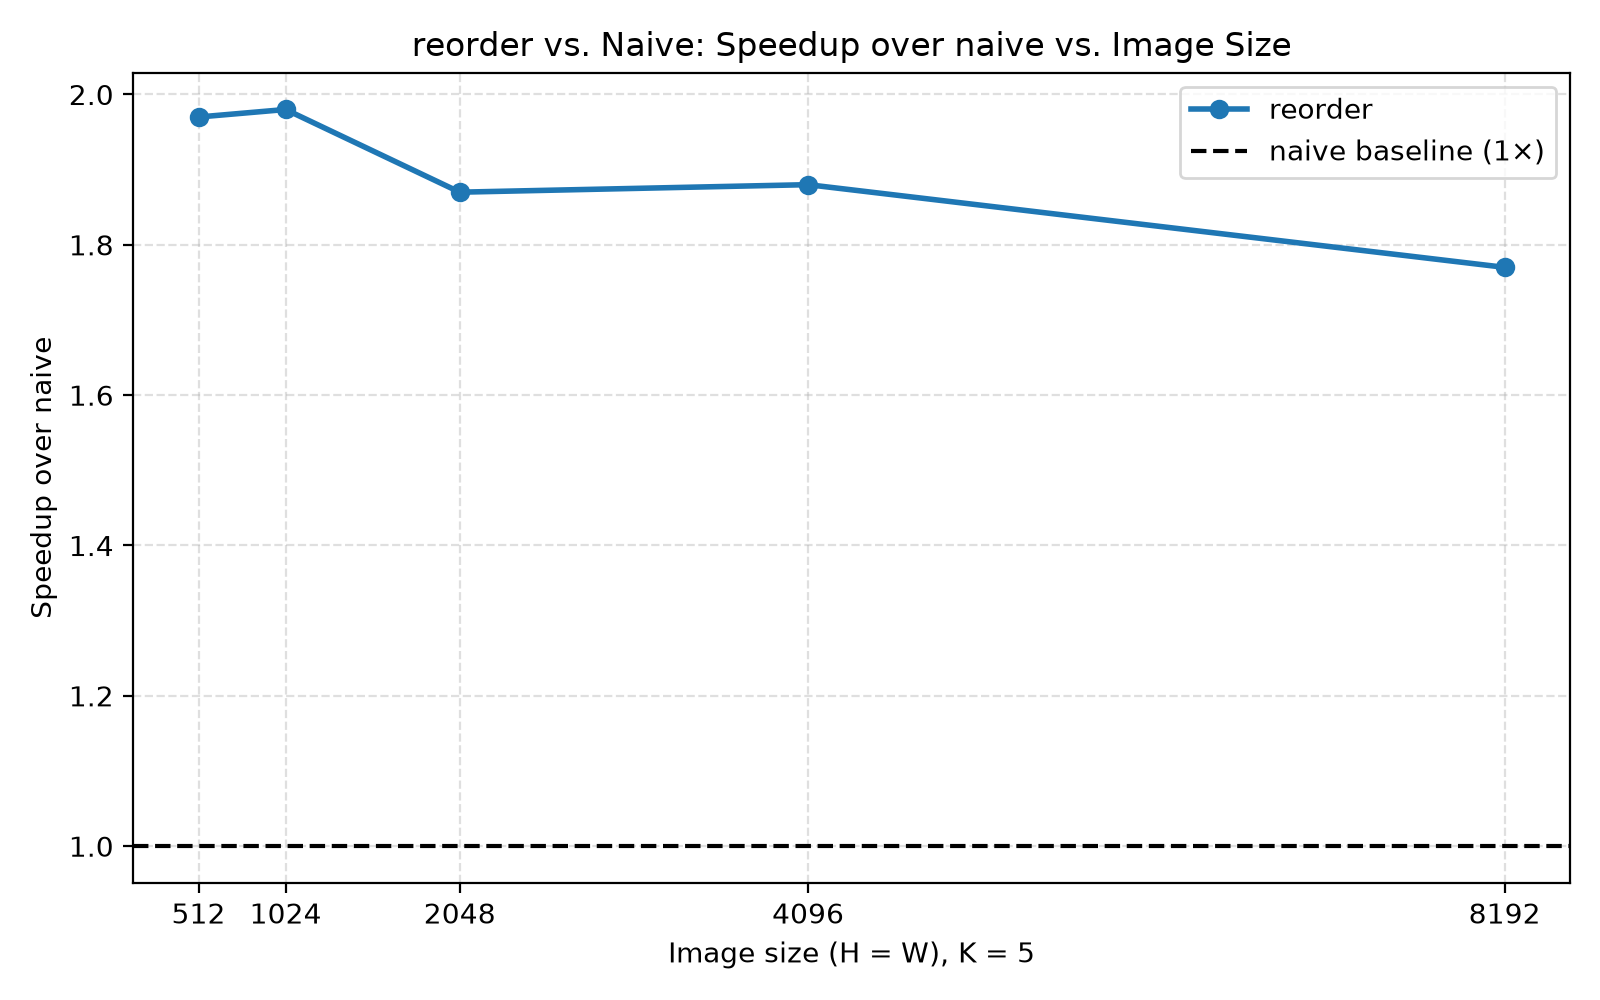
\includegraphics[width=\linewidth]{plots/task1a/reorder_vs_naive_speedup_image_size_k5.png}
        \caption{Reorder: Speedup vs. Image Size ($K=5$)}
        \label{fig:reorder_speedup_size}
    \end{subfigure}
    \hfill
    \begin{subfigure}{0.48\textwidth}
        \centering
        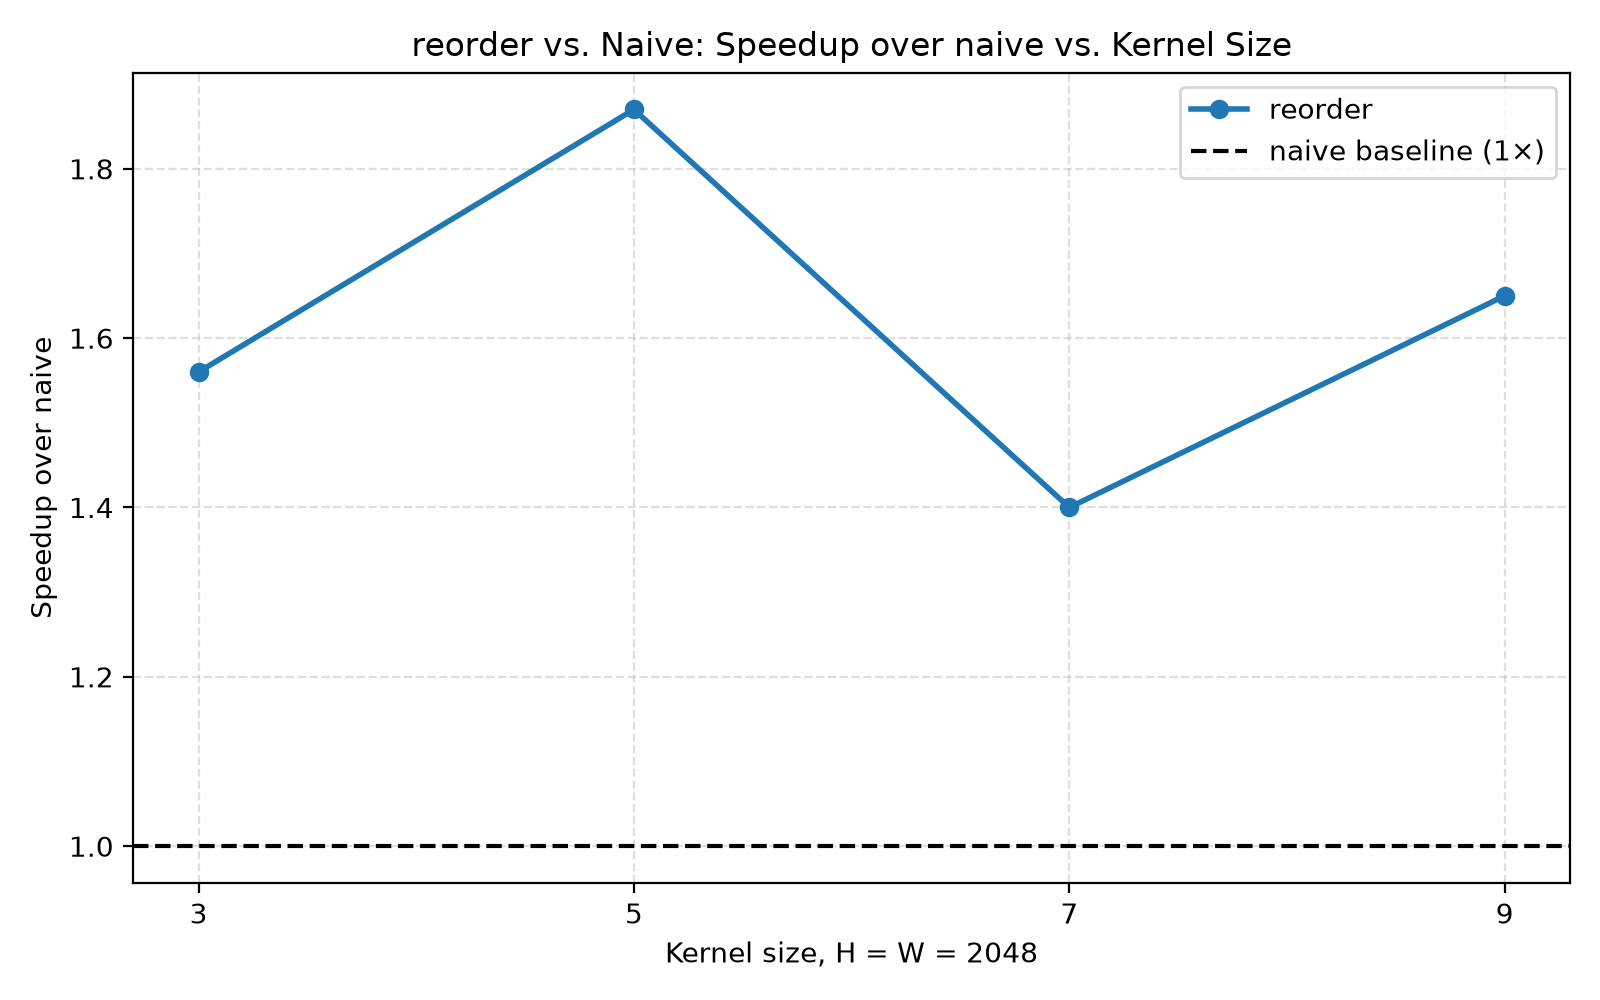
\includegraphics[width=\linewidth]{plots/task1a/reorder_vs_naive_speedup_kernel_size_2048.png}
        \caption{Reorder: Speedup vs. Kernel Size ($2048 \times 2048$)}
        \label{fig:reorder_speedup_kernel}
    \end{subfigure}
    
    \vspace{1em}
    \begin{subfigure}{0.48\textwidth}
        \centering
        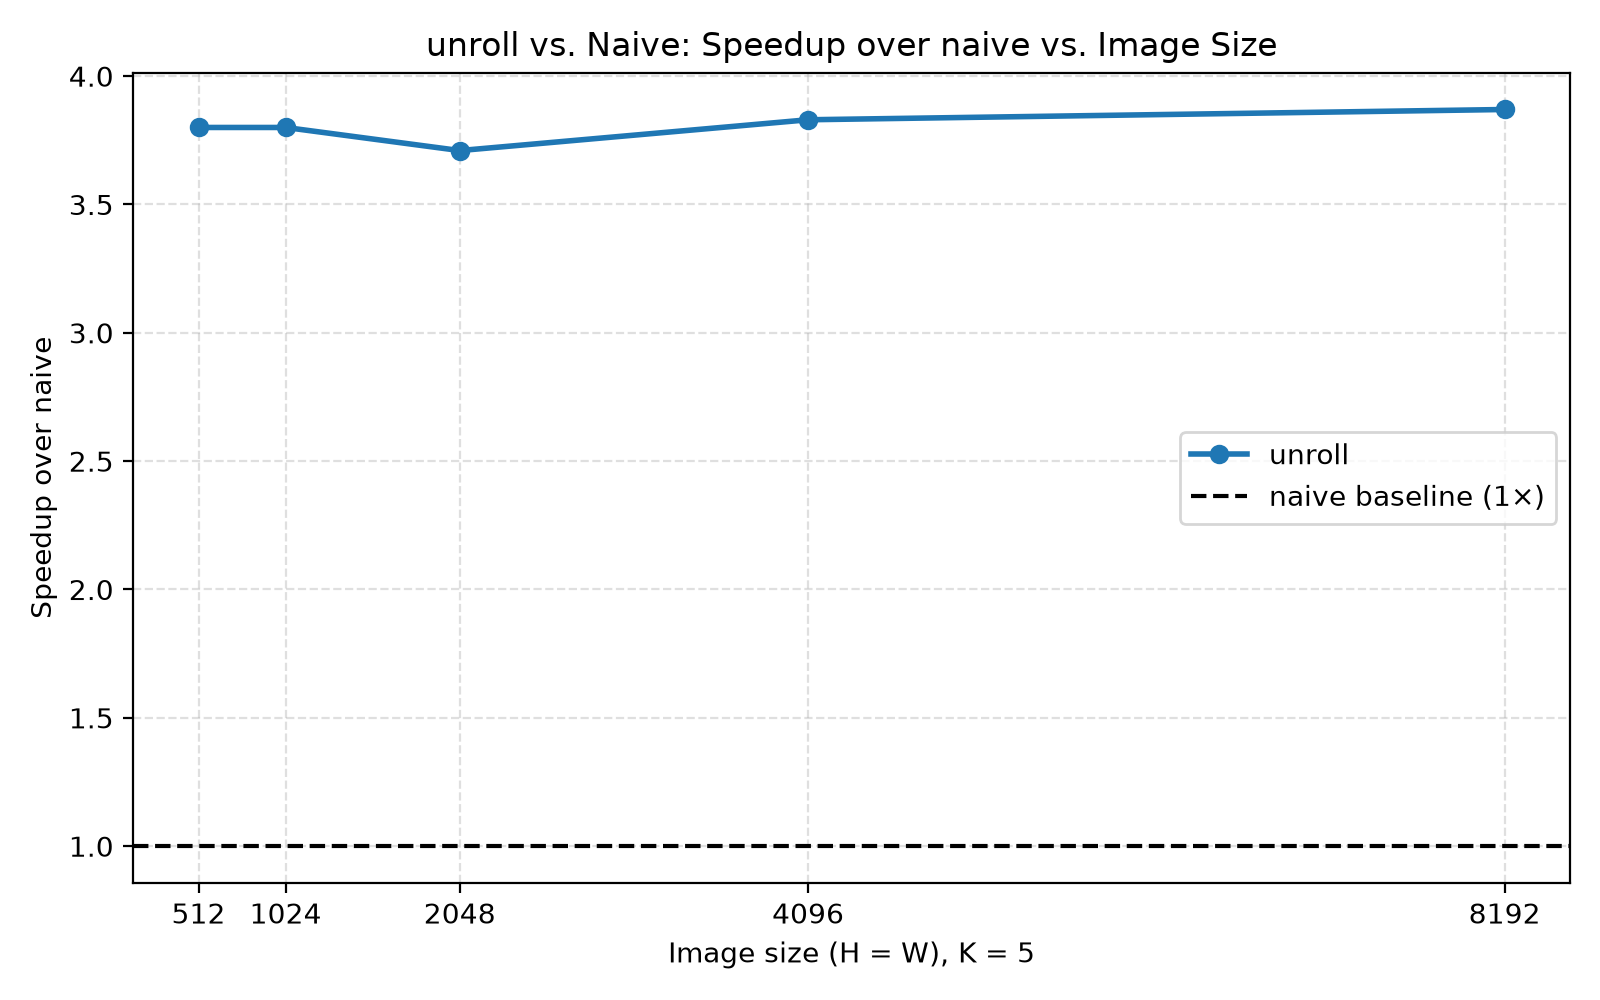
\includegraphics[width=\linewidth]{plots/task1a/unroll_vs_naive_speedup_image_size_k5.png}
        \caption{Unroll: Speedup vs. Image Size ($K=5$)}
        \label{fig:unroll_speedup_size}
    \end{subfigure}
    \hfill
    \begin{subfigure}{0.48\textwidth}
        \centering
        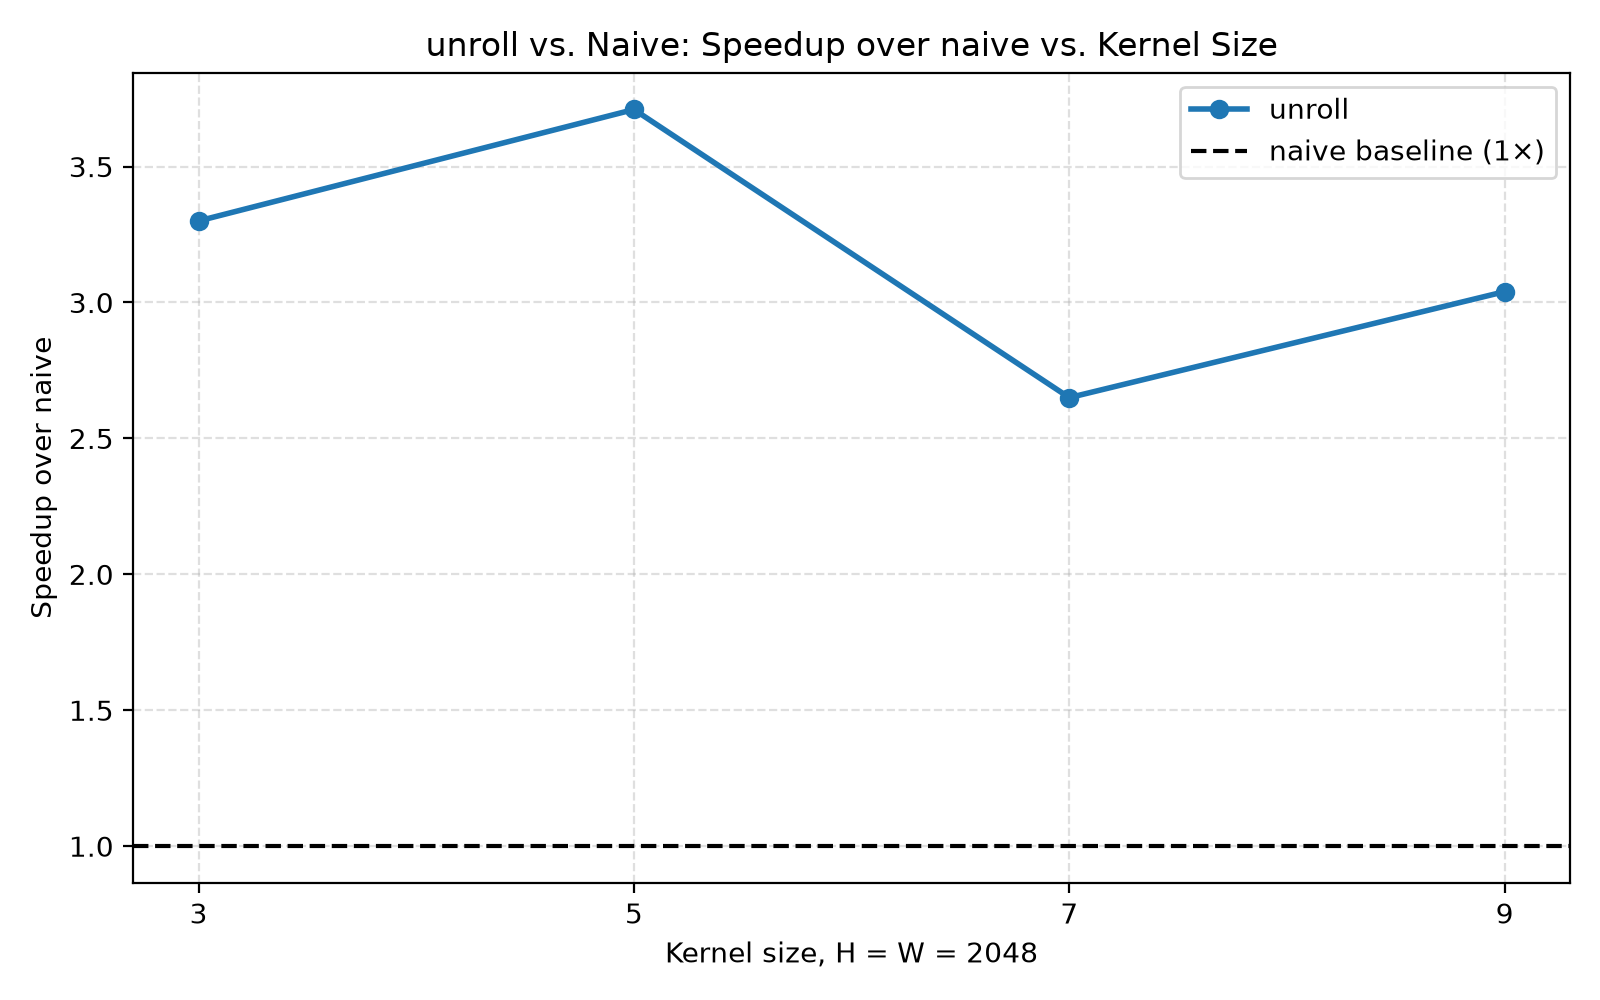
\includegraphics[width=\linewidth]{plots/task1a/unroll_vs_naive_speedup_kernel_size_2048.png}
        \caption{Unroll: Speedup vs. Kernel Size ($2048 \times 2048$)}
        \label{fig:unroll_speedup_kernel}
    \end{subfigure}
    \caption{Speedup performance comparisons against the naive baseline.}
    \label{fig:task1a_speedups}
\end{figure}

\subsection{Analysis}
Reordering yielded nearly a 2$\times$ speedup by making \texttt{ox} the innermost loop and increasing the useful work performed per fetched cache line. Unrolling resulted in an almost 4$\times$ speedup; the gain is consistent with both lower loop-control overhead and greater instruction-level parallelism from the independent accumulators.

As shown in Figure~\ref{fig:task1a_metrics}, unrolling drops instruction counts from $\sim$1.31 billion (naive) to $\sim$359 million (unrolled) for a $512 \times 512$ matrix. 

The total instruction counts for loop reordering remained comparable to the naive baseline but still the difference is significant and the performance is better. This suggests that for this case, we need to take into accoiunt both improved memory-access behavior as well as the instruction count reduction, rather than just one of them. 

\paragraph{Illustrating how Instruction Count Reduction via Reordering}While the primary goal of loop reordering is spatial cache locality, we observed that it also intrinsically reduces the total instruction count by minimizing loop maintenance overhead. This overhead consists of loop variable initialization, bounds checking, and incrementing. 

To illustrate, consider our spatial dimension ($2048$) and kernel dimension ($3$):
\begin{itemize}
    \item \textbf{Naive Ordering (Outer 2048, Inner 3):} The inner loop must be initialized $2048$ times. The outer loop evaluates its condition and increments $2048$ times.
    \item \textbf{Reordered (Outer 3, Inner 2048):} The inner loop is initialized only $3$ times. The outer loop evaluates its condition and increments only $3$ times.
\end{itemize}

By placing the spatial loops (\texttt{ox}) with massive bounds on the inside, and the kernel loops (\texttt{kx}) with tiny bounds on the outside, we drastically reduced the number of times the inner loops had to be set up and torn down. Across a full image convolution, this simple reordering inherently eliminates millions of redundant branch and initialization instructions, further contributing to the overall speedup.

\begin{figure}[H]
    \centering
    \begin{subfigure}{0.48\textwidth}
        \centering
        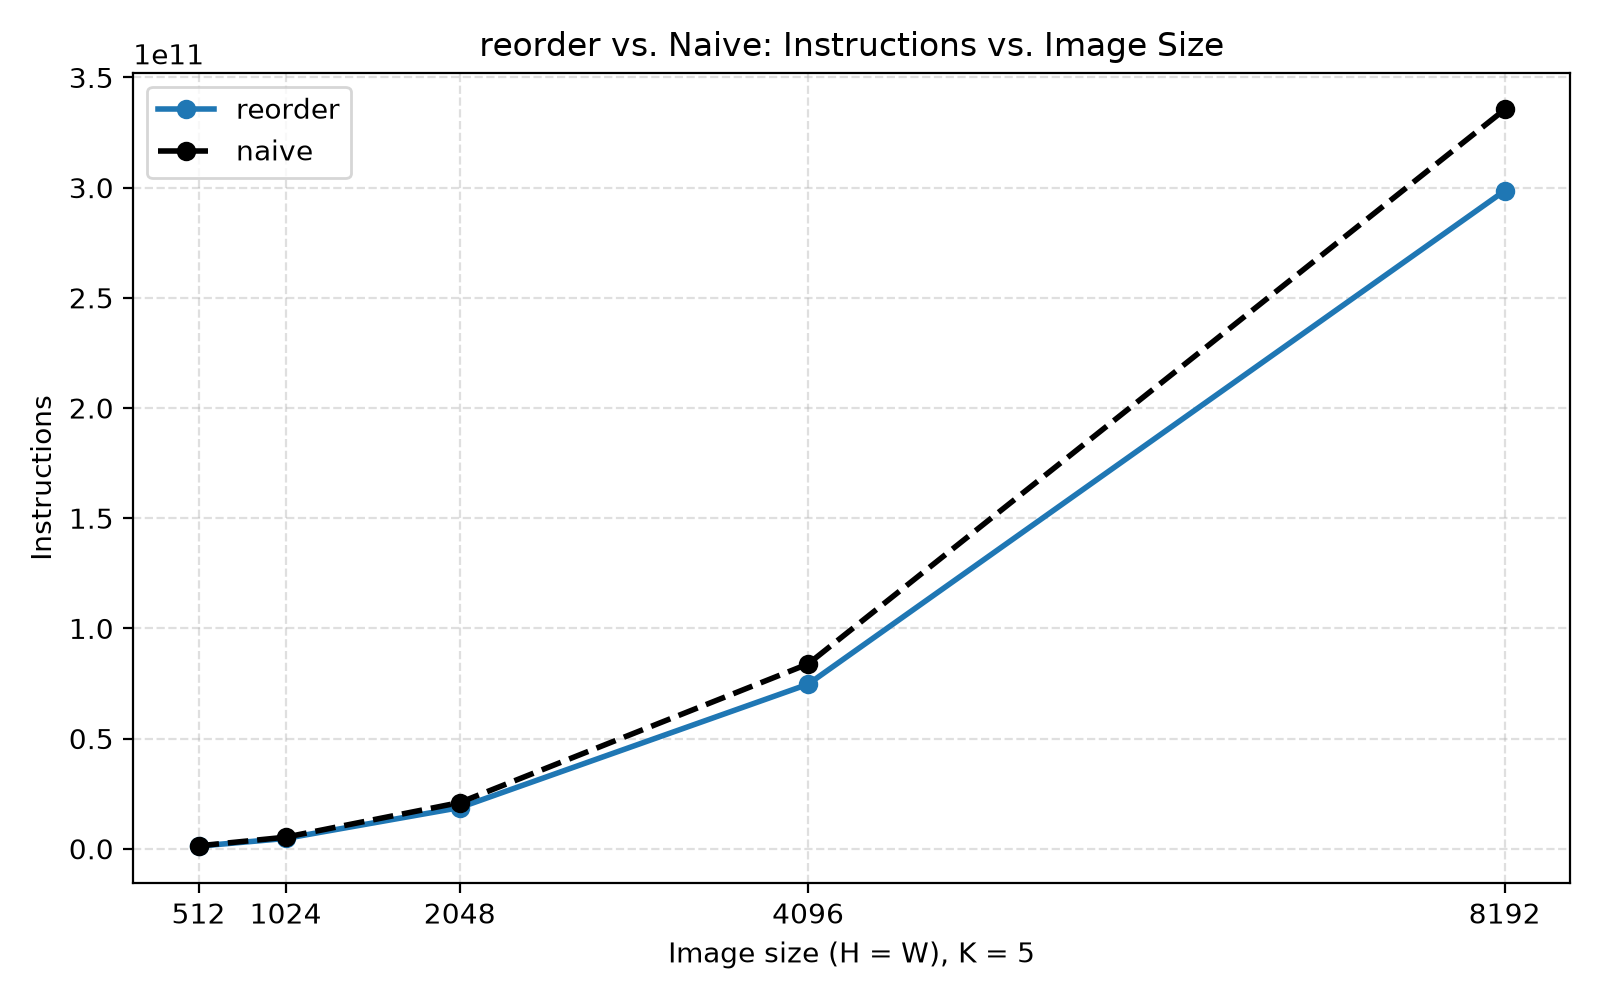
\includegraphics[width=\linewidth]{plots/task1a/reorder_vs_naive_instructions_image_size_k5.png}
        \caption{Reorder: Instructions vs. Image Size ($K=5$)}
    \end{subfigure}
    \hfill
    \begin{subfigure}{0.48\textwidth}
        \centering
        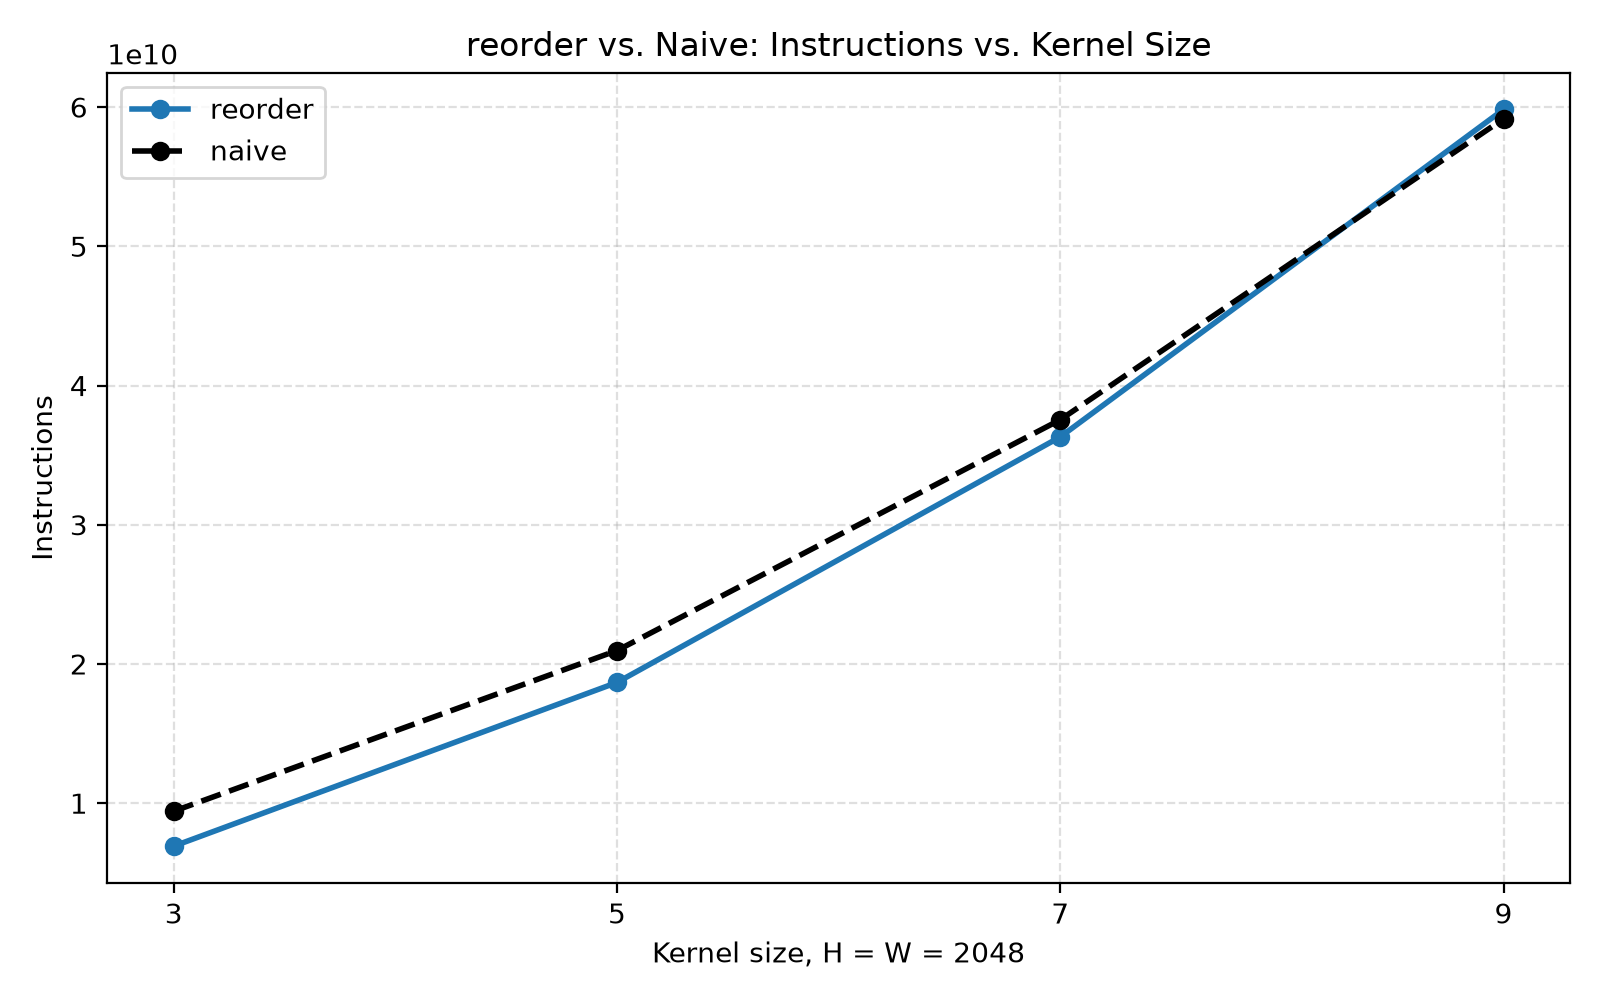
\includegraphics[width=\linewidth]{plots/task1a/reorder_vs_naive_instructions_kernel_size_2048.png}
        \caption{Reorder: Instructions vs. Kernel Size ($2048 \times 2048$)}
    \end{subfigure}
    
    \vspace{1em}
    \begin{subfigure}{0.48\textwidth}
        \centering
        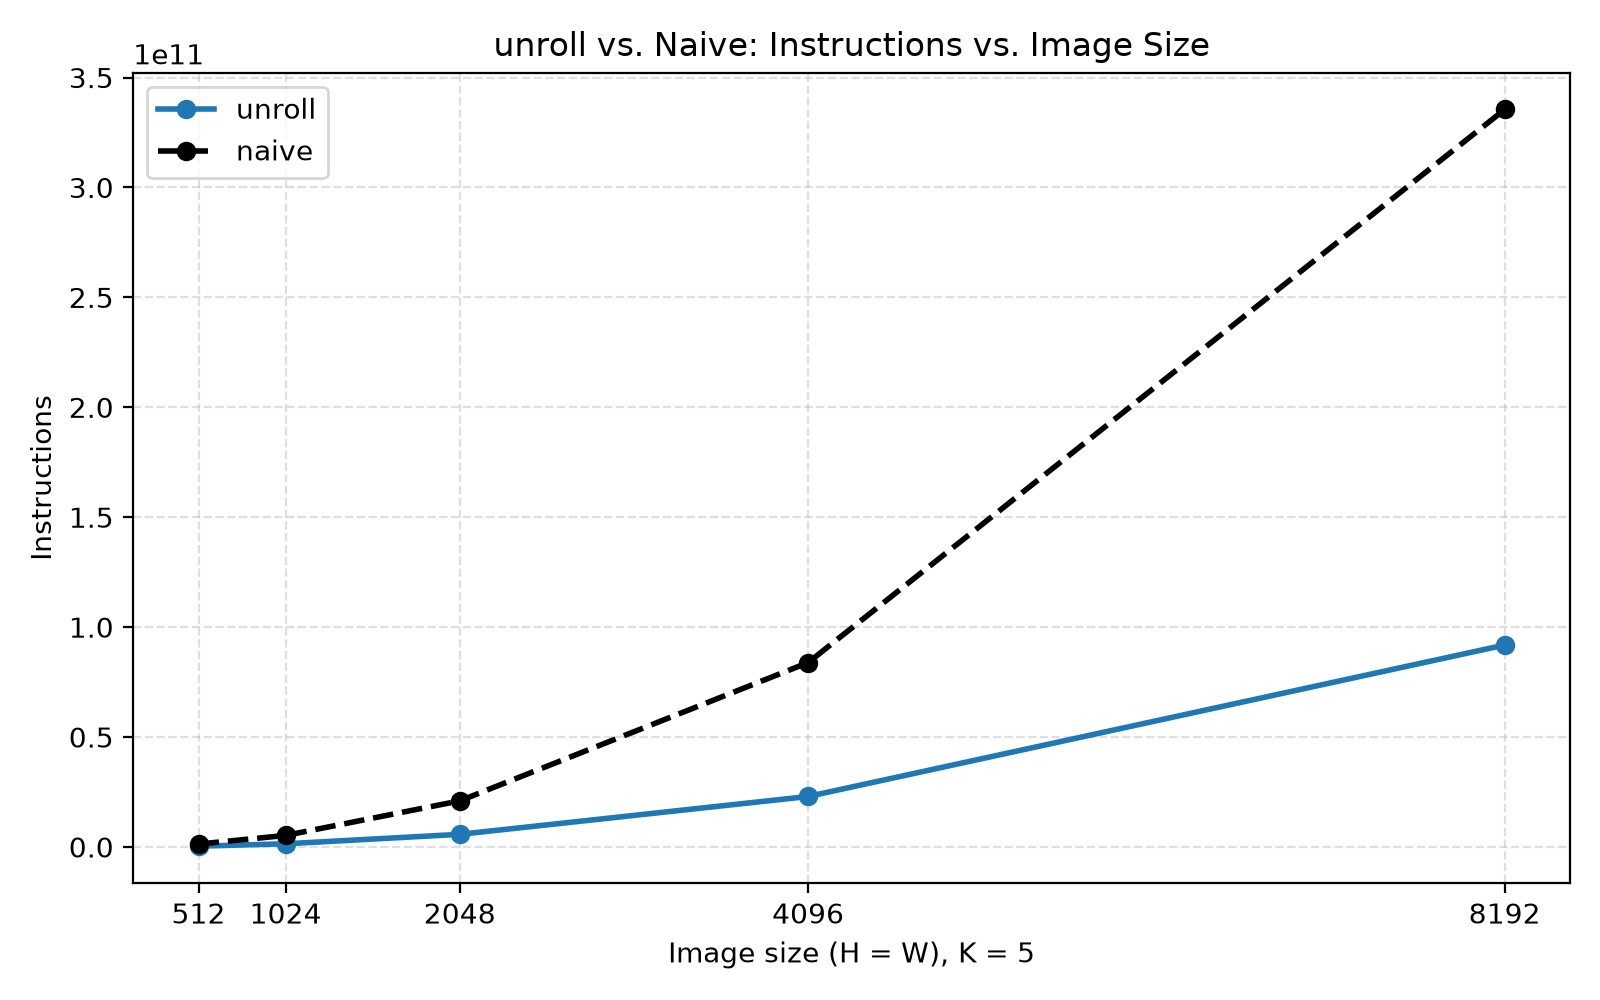
\includegraphics[width=\linewidth]{plots/task1a/unroll_vs_naive_instructions_image_size_k5.png}
        \caption{Unroll: Instructions vs. Image Size ($K=5$)}
    \end{subfigure}
    \hfill
    \begin{subfigure}{0.48\textwidth}
        \centering
        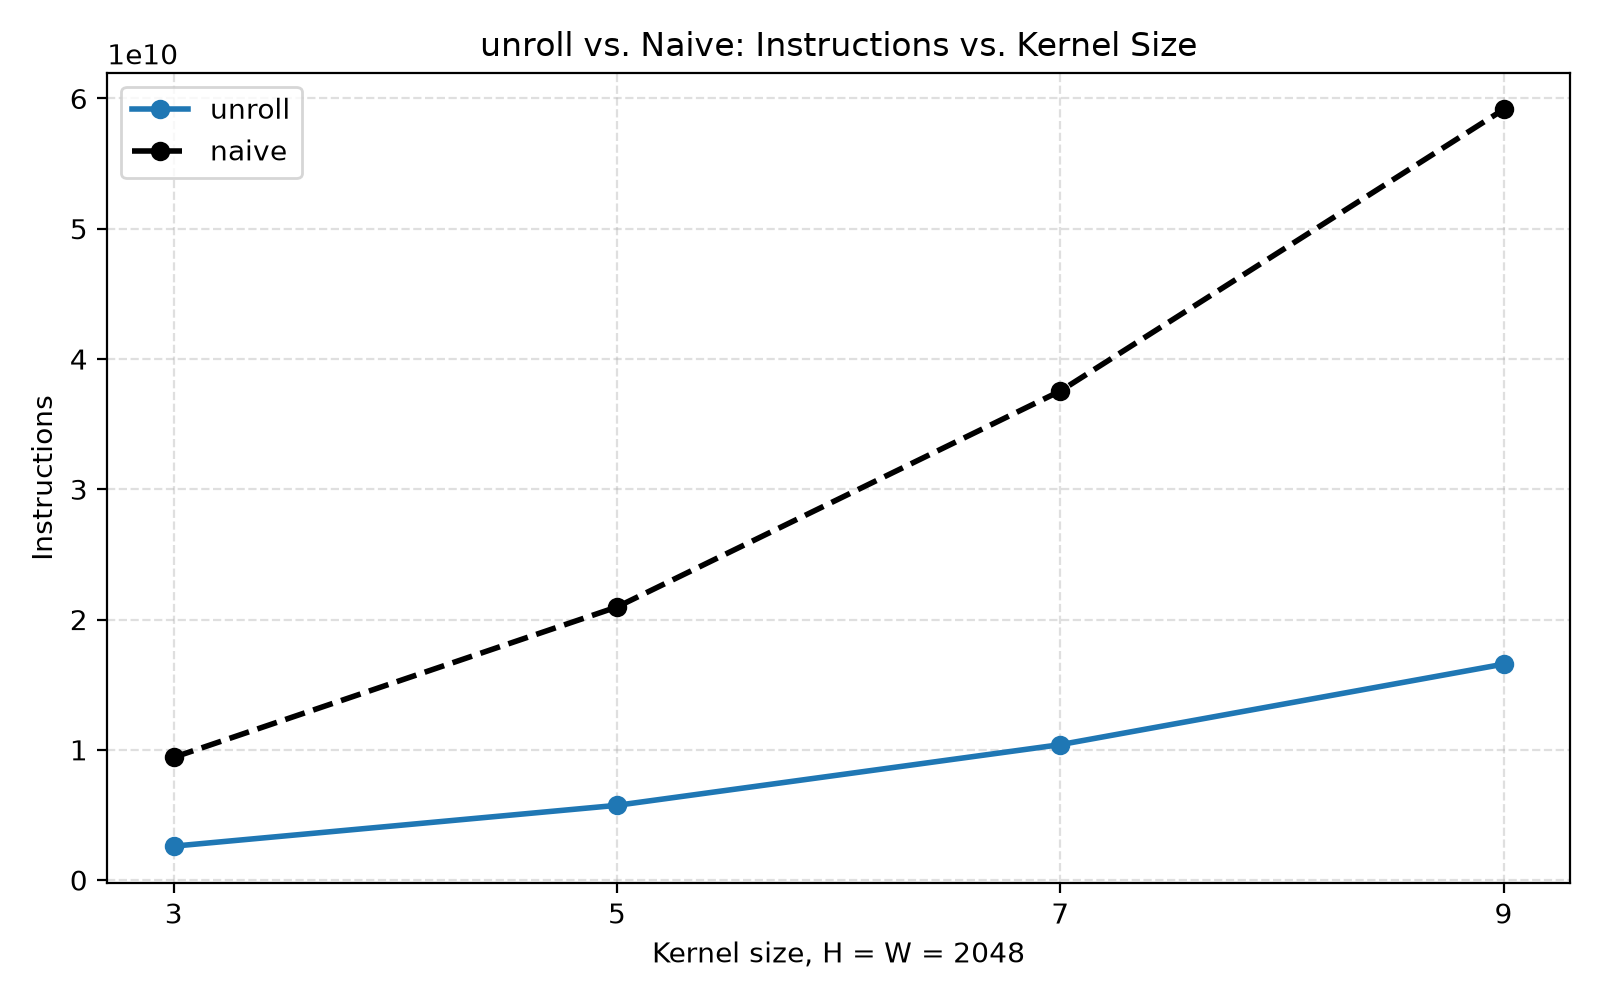
\includegraphics[width=\linewidth]{plots/task1a/unroll_vs_naive_instructions_kernel_size_2048.png}
        \caption{Unroll: Instructions vs. Kernel Size ($2048 \times 2048$)}
    \end{subfigure}

    \vspace{1em}
    \begin{subfigure}{0.48\textwidth}
        \centering
        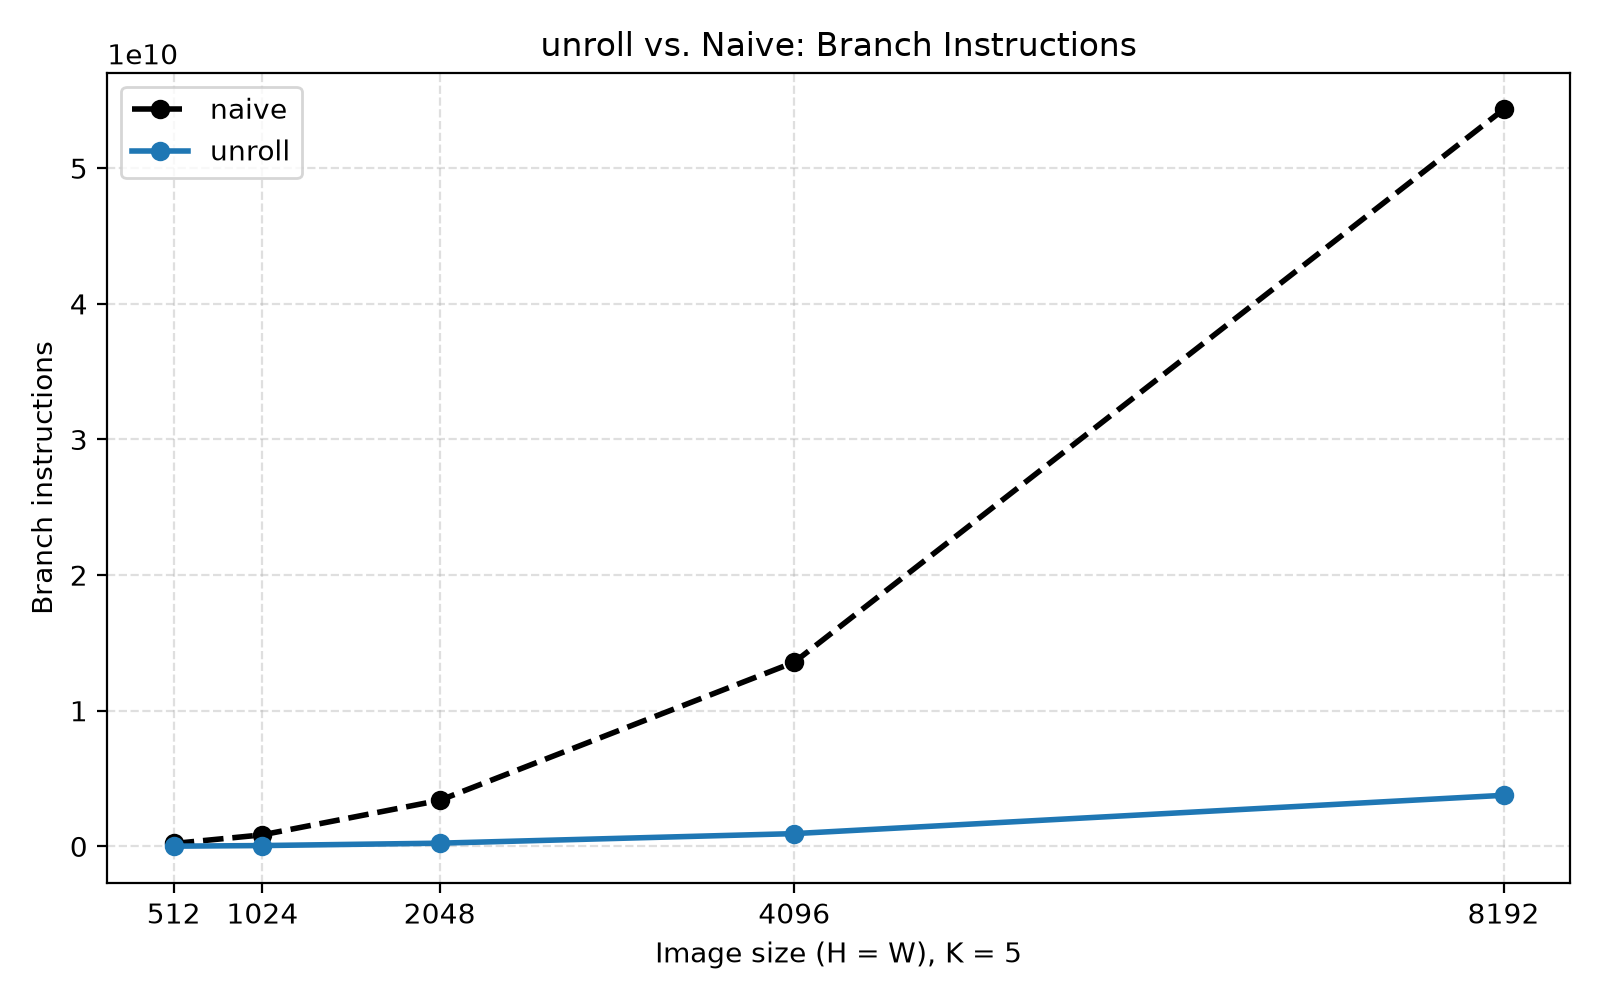
\includegraphics[width=\linewidth]{plots/task1a/unroll_vs_naive_branches_image_size_k5.png}
        \caption{Unroll: Branches vs. Image Size ($K=5$)}
    \end{subfigure}
    \hfill
    \begin{subfigure}{0.48\textwidth}
        \centering
        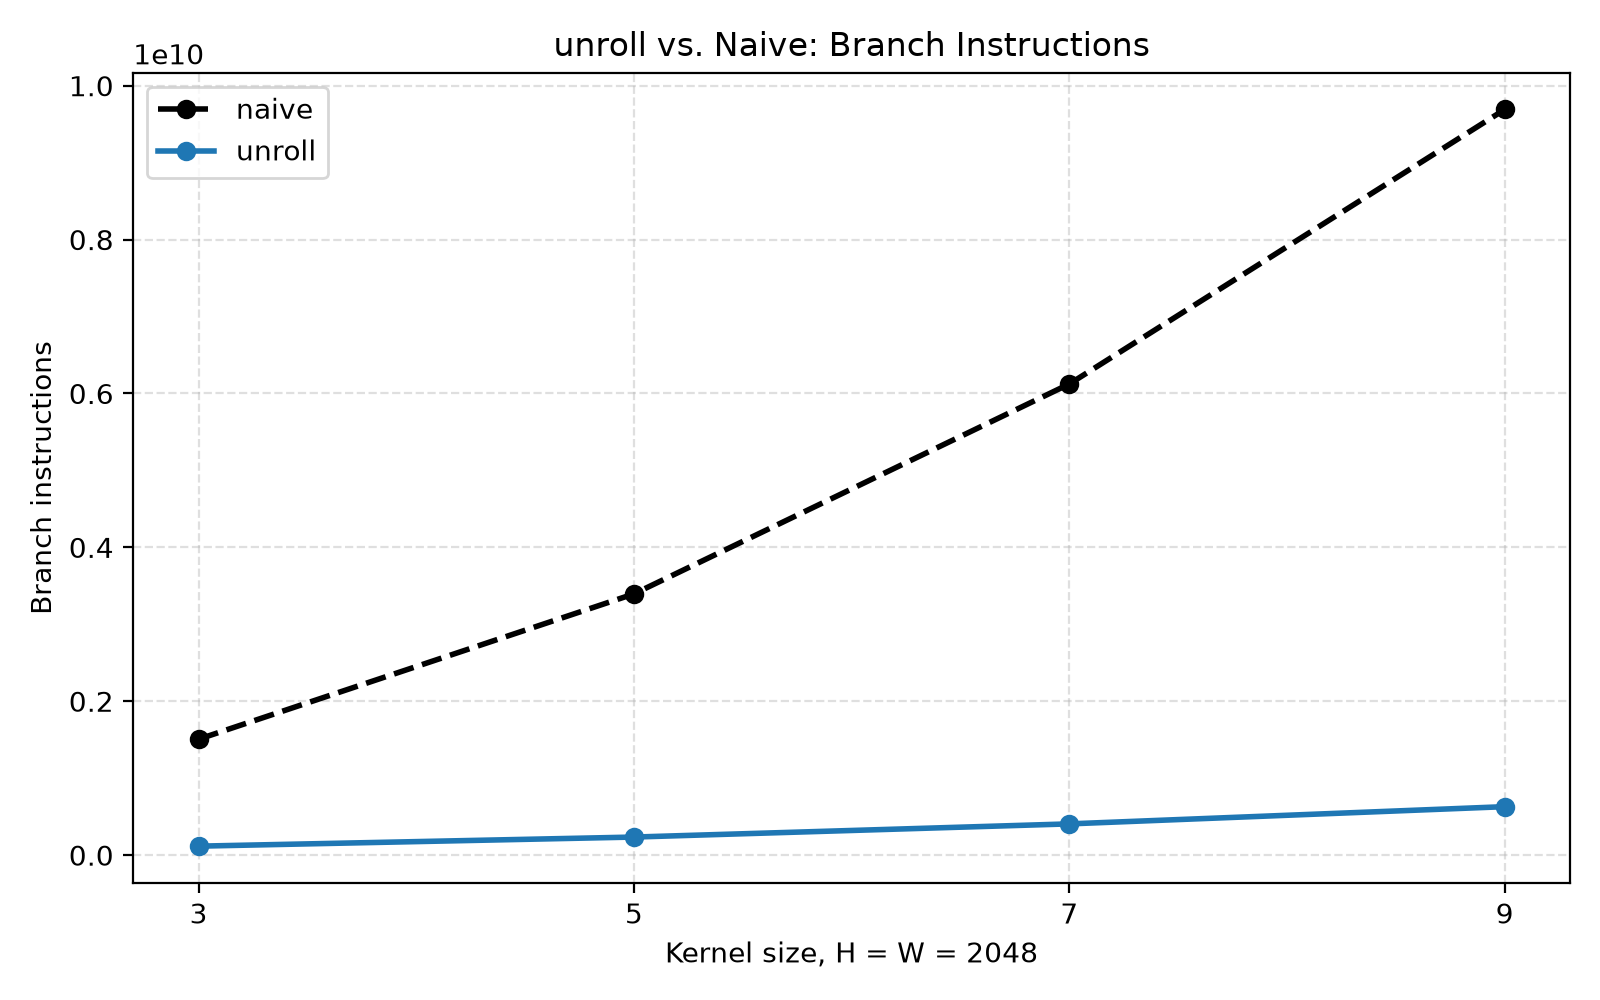
\includegraphics[width=\linewidth]{plots/task1a/unroll_vs_naive_branches_kernel_size_2048.png}
        \caption{Unroll: Branches vs. Kernel Size ($2048 \times 2048$)}
    \end{subfigure}
    \caption{Hardware instruction and branch metrics demonstrating loop overhead reduction.}
    \label{fig:task1a_metrics}
\end{figure}

\subsection{Questions}
\begin{enumerate}
    \item \textbf{What motivated you to make changes to the code?} \\
    To reduce loop-control work and improve reuse across adjacent output pixels; the baseline already has contiguous accesses along \texttt{kx}, but its overall loop order does not expose this reuse as effectively.
    \item \textbf{What considerations did you take into account?} \\
    I prioritized contiguous spatial memory access (reordering) and balanced the unroll factor (8 for spatial width) to fully utilize registers without spilling.
    \item \textbf{How effective were the changes? Which metric was used and why?} \\
    Effective (up to 3.87$\times$ speedup). Execution time was used for raw performance, while instruction counts and branch metrics support the interpretation that unrolling reduces loop overhead and exposes independent work.
\end{enumerate}

% ============================================================
% 1B: Tiling
% ============================================================

\subsection{Task 1B: Tiling}

\subsubsection{Baseline Profiling}
The L1 Data (L1-D) cache size on the tested system is 448 KiB. Profiling the baseline (naive) 2D convolution yields an L1-D MPKI of 0.06 for a 2048x2048 matrix with a kernel size of 5.

\subsubsection{Implementation}
The tiled 2D convolution is implemented by dividing the output matrix into square blocks of a fixed dimension, \texttt{sz}[cite: 5]. The outer loops iterate over the tile origins (\texttt{oyT} and \texttt{oxT}) to process the image block by block[cite: 5]. Within each tile block, the output values are initialized to zero, and the kernel loops (\texttt{ky} and \texttt{kx}) accumulate the weighted inputs strictly within the local spatial bounds[cite: 5]. This reorders the memory accesses to keep the active working set confined within the cache.

\begin{figure}[H]
    \centering
    \begin{subfigure}{0.48\textwidth}
        \centering
        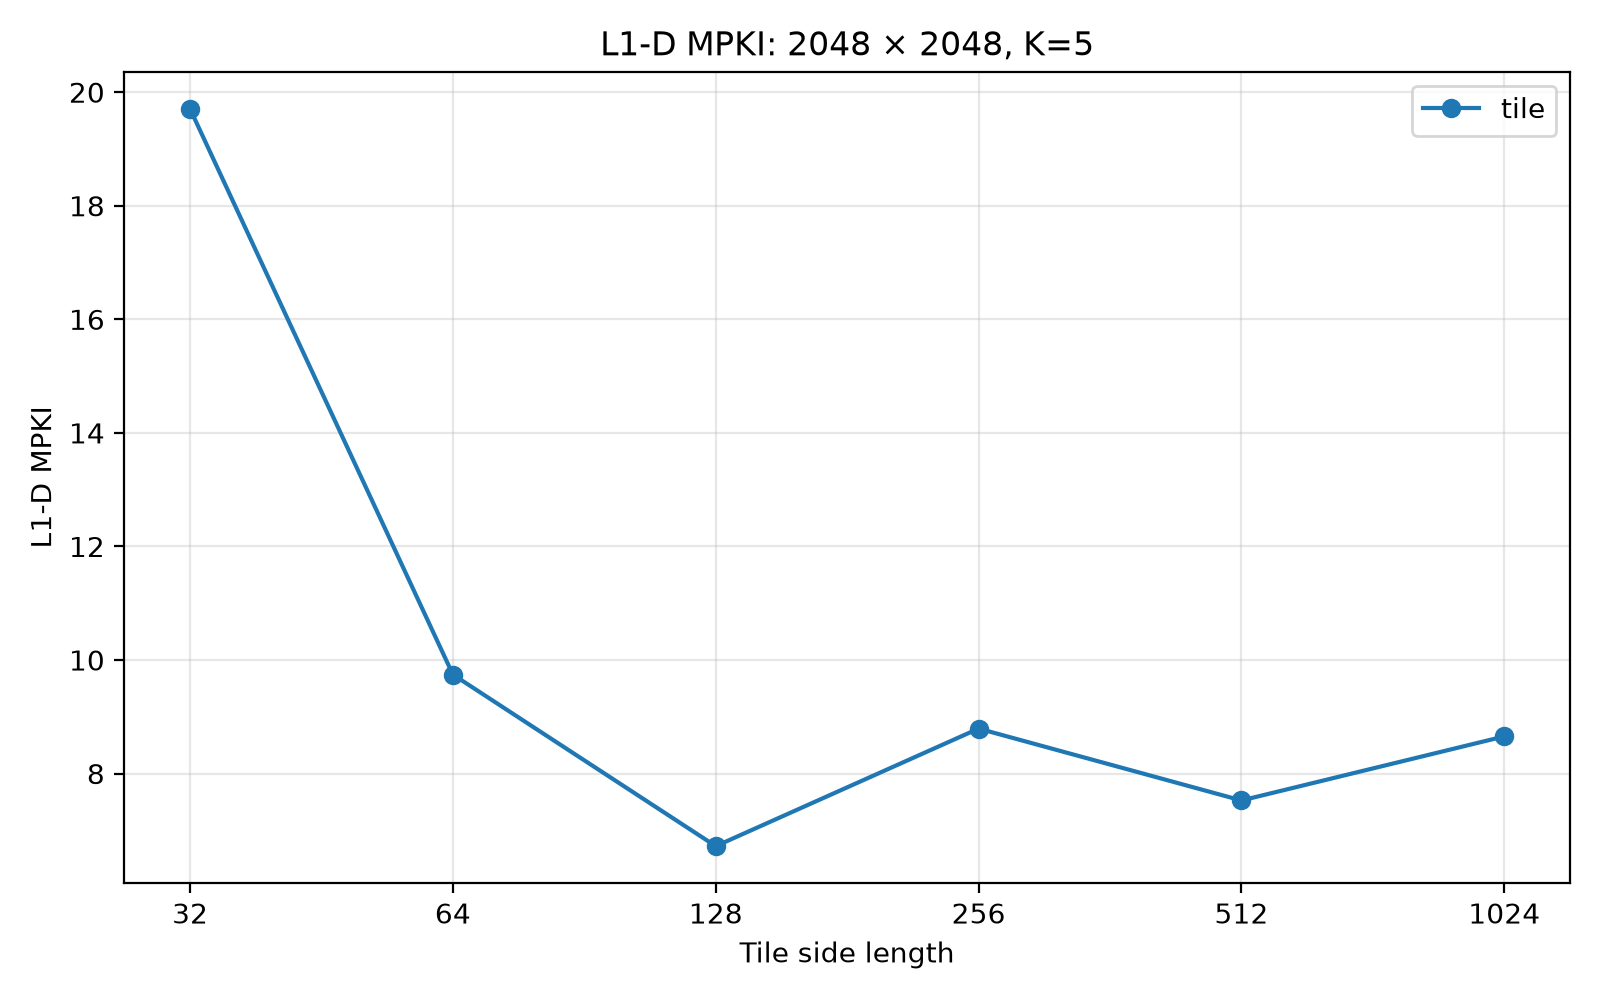
\includegraphics[width=\linewidth]{plots/task1b/plots_1d/n2048_l1_mpki_k5.png}
        \caption{L1-D MPKI vs. Tile Size (2048x2048)}
        \label{fig:tiling_mpki_1d}
    \end{subfigure}
    \hfill
    \begin{subfigure}{0.48\textwidth}
        \centering
        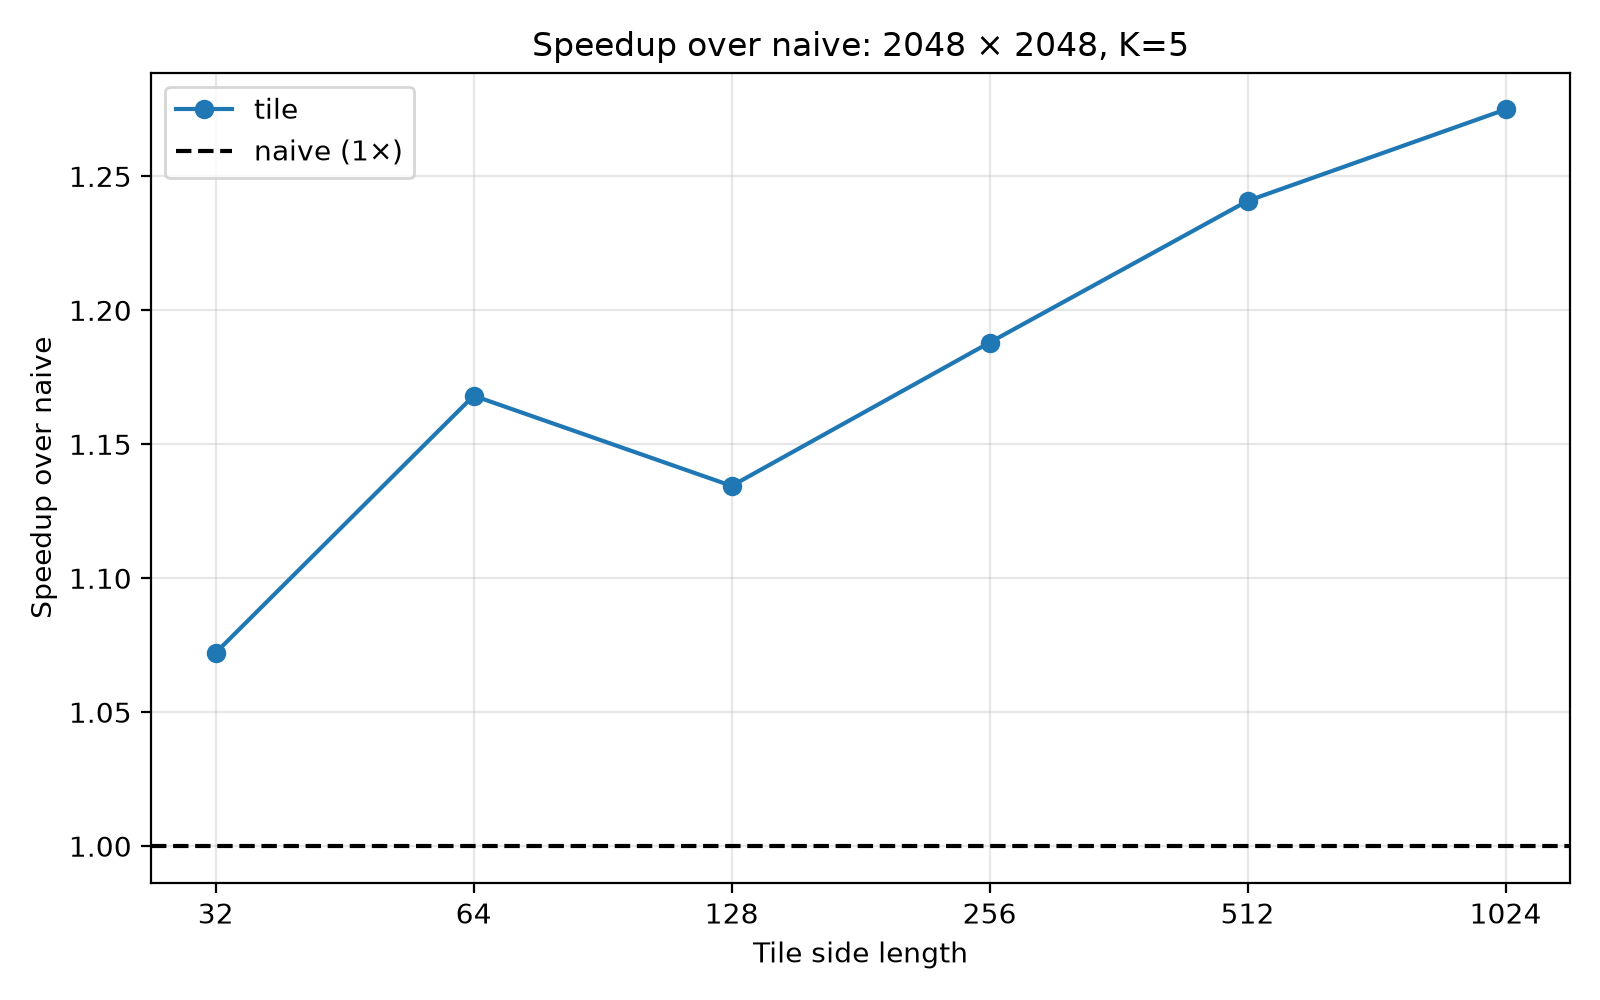
\includegraphics[width=\linewidth]{plots/task1b/plots_1d/n2048_speedup_k5.png}
        \caption{Speedup vs. Tile Size (2048x2048)}
        \label{fig:tiling_speedup_1d}
    \end{subfigure}
    \caption{Cache behavior and performance for a 2048x2048 matrix at $K=5$.}
    \label{fig:task1b_1d}
\end{figure}

\begin{figure}[H]
    \centering
    \begin{subfigure}{0.48\textwidth}
        \centering
        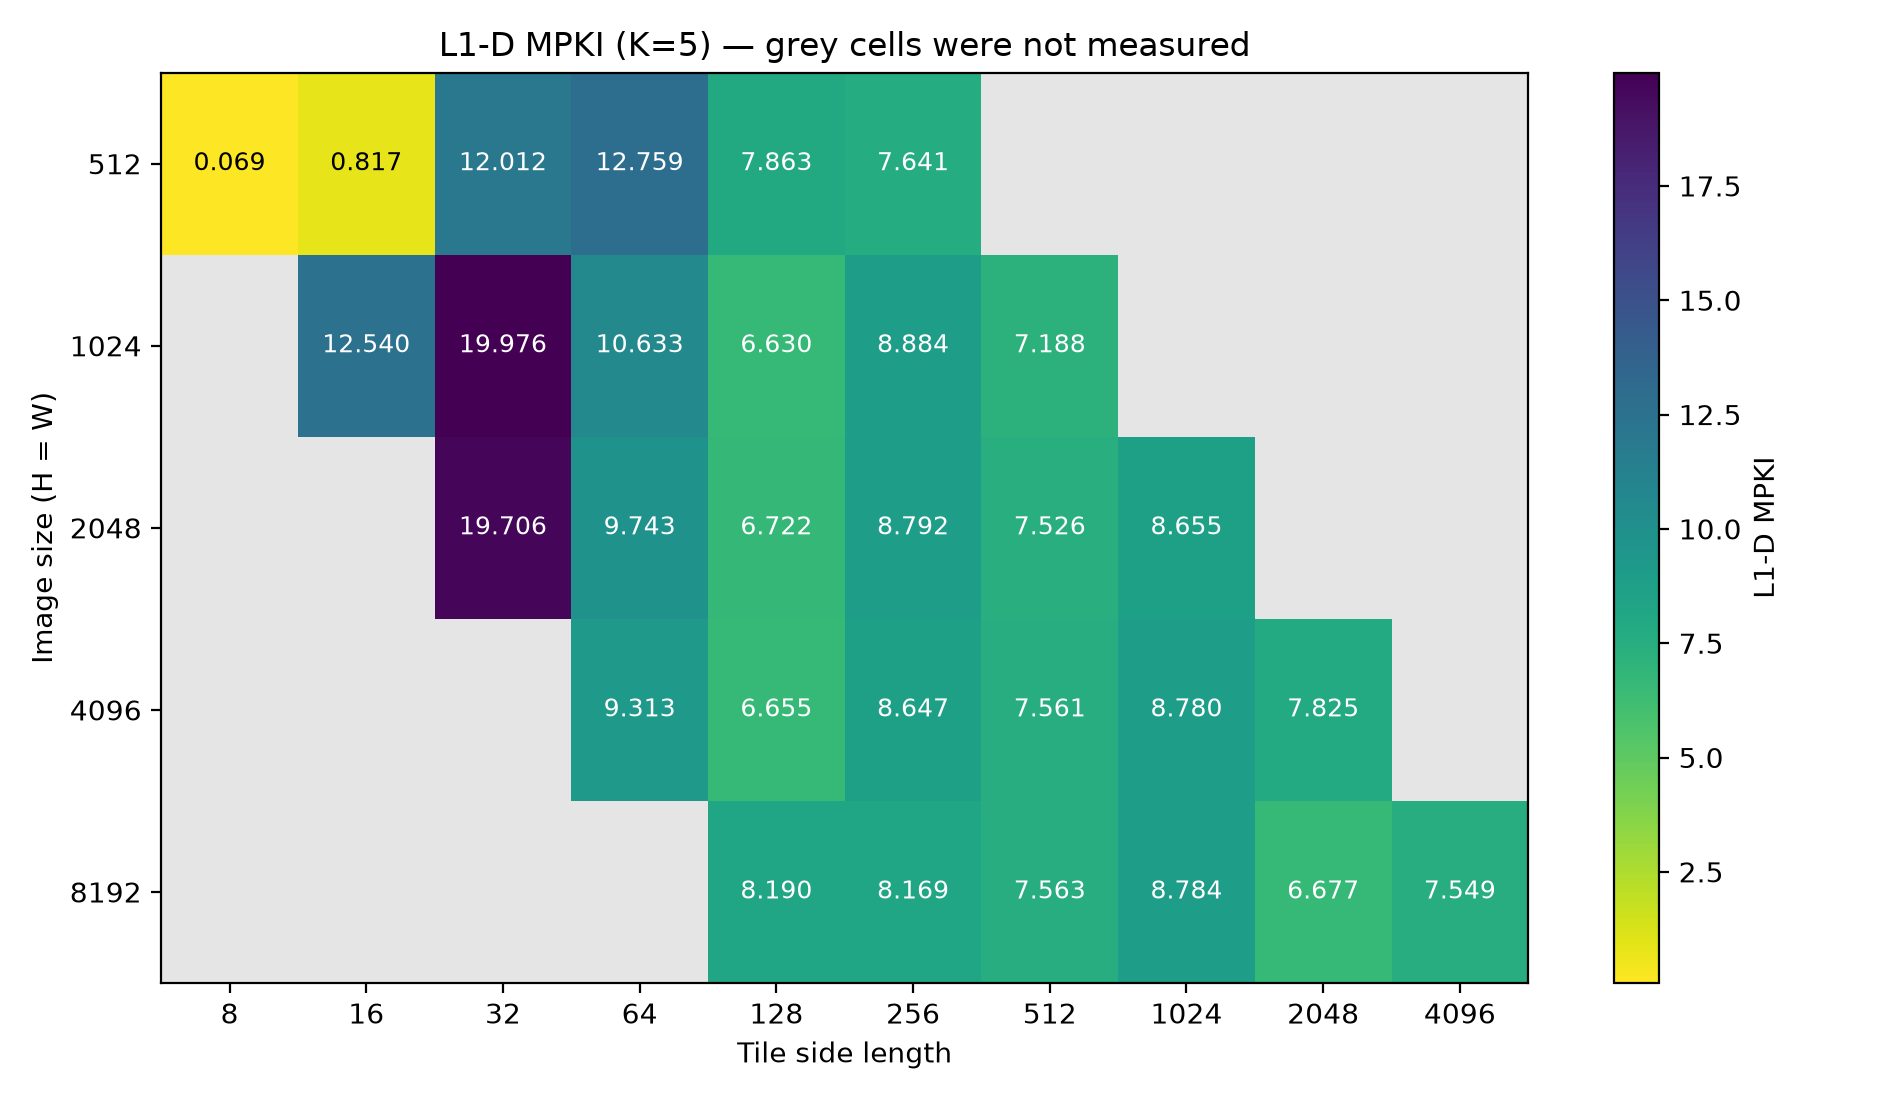
\includegraphics[width=\linewidth]{plots/task1b/plots_2d/l1_mpki_heatmap_k5.png}
        \caption{L1-D MPKI Heatmap}
        \label{fig:tiling_mpki_heatmap}
    \end{subfigure}
    \hfill
    \begin{subfigure}{0.48\textwidth}
        \centering
        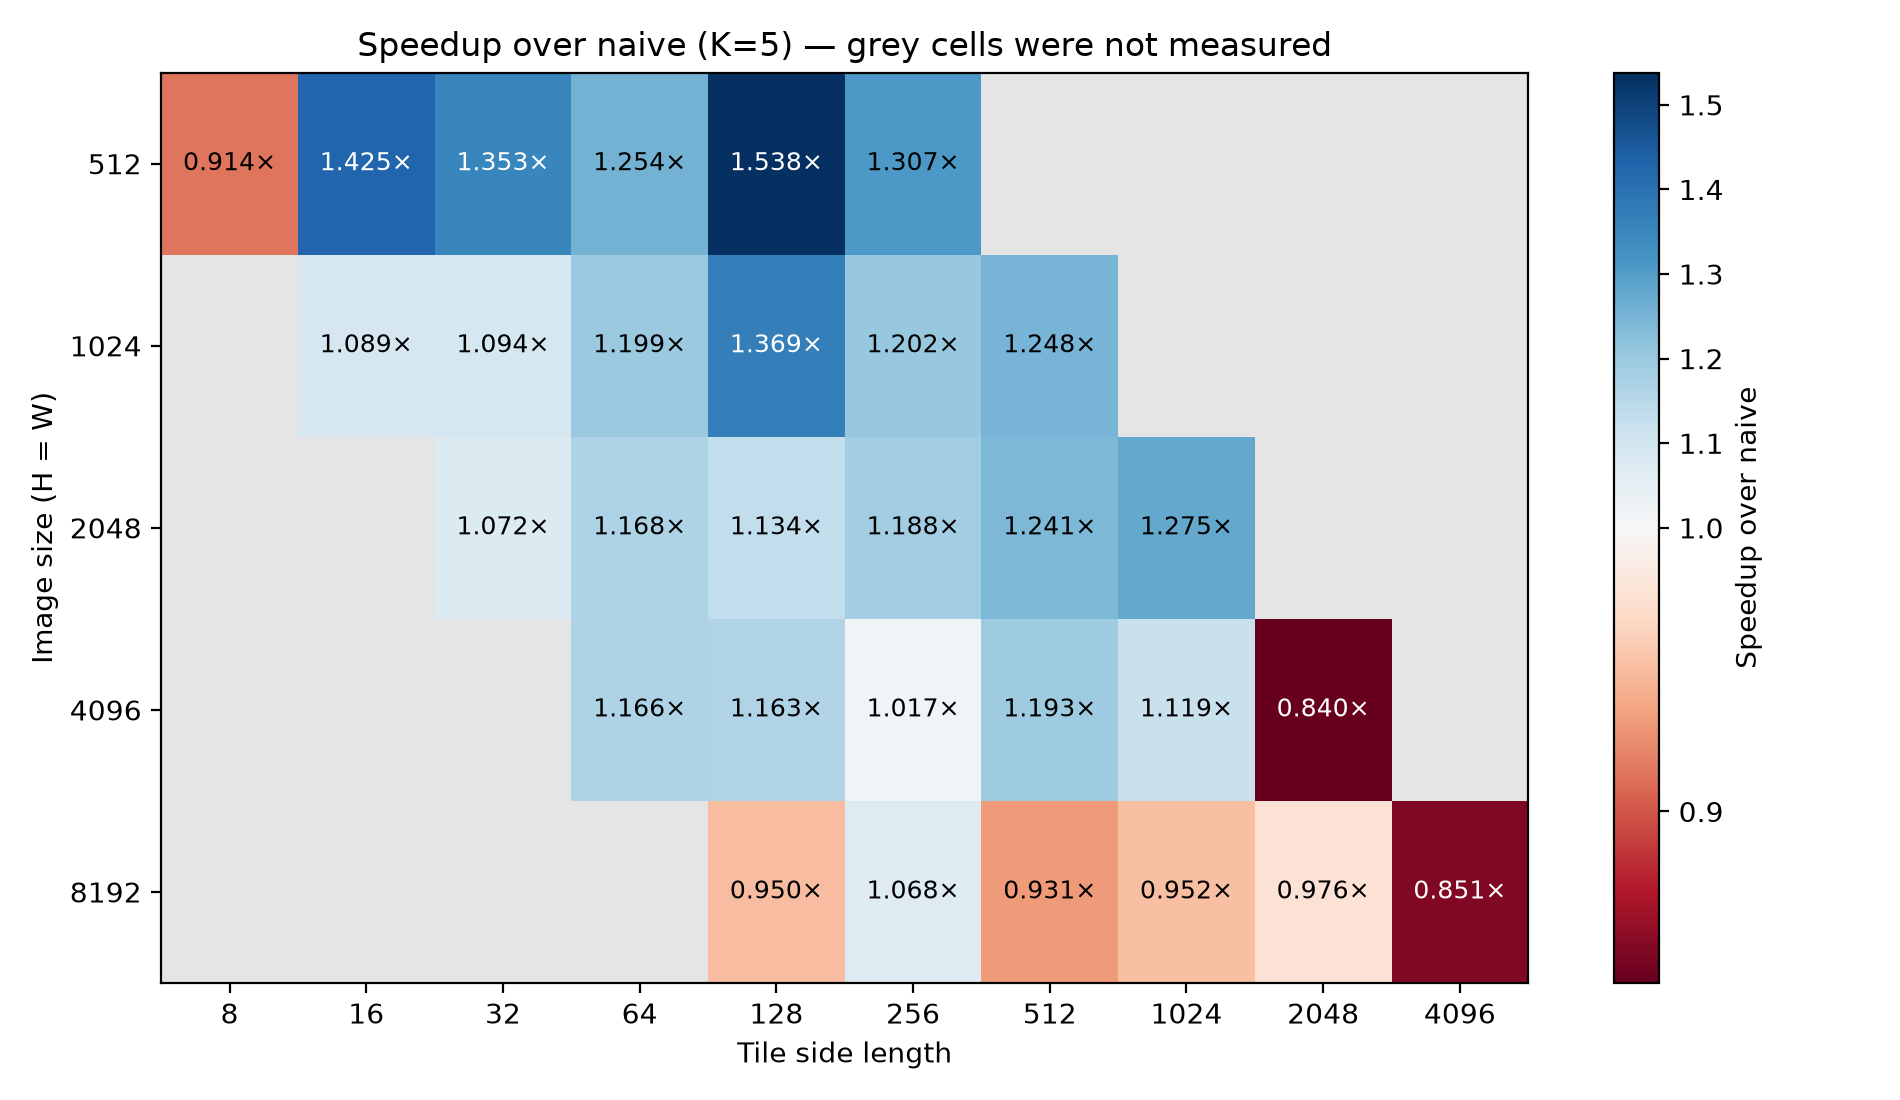
\includegraphics[width=\linewidth]{plots/task1b/plots_2d/speedup_heatmap_k5.png}
        \caption{Speedup Heatmap}
        \label{fig:tiling_speedup_heatmap}
    \end{subfigure}
    \caption{Performance trends across varying matrix sizes and tile sizes ($K=5$).}
    \label{fig:task1b_2d}
\end{figure}

\subsubsection{Analysis}

\begin{enumerate}
    \item \textbf{Report the changes in L1-D MPKI observed when moving from naive to tiled 2D convolution. Justify your observations.} \\
    The L1-D MPKI increased significantly, jumping from just 0.06 in the naive version to a range of $\sim$6 to 19 in the tiled version. The naive implementation accesses memory in long, predictable linear streams, which hardware prefetchers can easily identify and hide. Tiling breaks these accesses into short, discontinuous blocks, which disrupts the hardware prefetchers and exposes the actual cache miss rate.
    
    \item \textbf{How did L1-D MPKI vary across different matrix sizes and tile sizes? Explain your findings in terms of the cache hierarchy and working set sizes.} \\
    MPKI hits a minimum at intermediate "sweet spot" tile sizes (e.g., 128 for a 2048x2048 matrix). If the tile size is too large (e.g., $\ge$ 512), the working set memory footprint exceeds the system's 448 KiB L1 cache capacity, resulting in capacity misses. If the tile size is too small (e.g., 32), the boundary overhead and frequent pointer jumps increase the relative miss rate without providing additional cache benefits.
    
    \item \textbf{Did you achieve a speedup? If yes, quantify the improvement and identify the contributing factors. If not, analyze the limiting factors and propose possible solutions.} \\
    Yes, a speedup was achieved. For a 2048x2048 matrix, the speedup reached $\sim$1.27$\times$ at a tile size of 1024, and peaked at 1.53$\times$ for a 512x512 matrix with a tile size of 256. Despite the higher L1-D MPKI caused by prefetcher disruption, overall execution time improved because tiling maximizes data reuse in the larger L2 and Last Level Caches (LLC), significantly reducing the high latency penalty of fetching data from main memory.
\end{enumerate}
% ============================================================
% 1C
% ============================================================

\section{Task 1C: SIMD}

\subsection{Baseline Instruction Count}
For a $512 \times 512$ matrix with a kernel size of $K=5$, the naive baseline implementation executed $\sim$1.31 billion instructions.

\subsection{SIMD Implementations}
The convolution algorithm was parallelized using Intel AVX intrinsics . The inner spatial loop was stepped by the SIMD vector width (e.g., 8 floats for 256-bit AVX2) . Both 128-bit (SSE) and 256-bit (AVX2) implementations were evaluated across different matrix sizes to measure vectorization efficiency.

\begin{table}[H]
\centering
\caption{Task 1C SIMD results ($K=5$)}
\begin{tabular}{lcccc}
\toprule
Matrix Size & SIMD Width & Instructions & Time (ms) & Speedup \\
\midrule
$512 \times 512$   & 128-bit & 296,643,371   & 0.466 & 8.40$\times$ \\
$512 \times 512$   & 256-bit & 158,009,805   & 0.522 & 7.95$\times$ \\
$1024 \times 1024$ & 128-bit & 1,183,171,431 & 2.175 & 7.10$\times$ \\
$1024 \times 1024$ & 256-bit & 628,631,602   & 2.189 & 7.74$\times$ \\
$2048 \times 2048$ & 256-bit & 2,510,515,355 & 9.150 & 7.47$\times$ \\
\bottomrule
\end{tabular}
\end{table}

\subsection{SIMD Intrinsics}

\begin{itemize}
    \item \texttt{\_mm256\_setzero\_ps}: Purpose: Initializes a 256-bit accumulator vector to zero . Justification: Needed to clear the parallel accumulator state before summing the kernel convolution .
    \item \texttt{\_mm256\_loadu\_ps} / \texttt{\_mm256\_storeu\_ps}: Purpose: Loads/stores 8 contiguous floats to/from memory. Unaligned loads and stores were used because 32-byte alignment cannot be guaranteed for every accessed address.
    \item \texttt{\_mm256\_set1\_ps}: Purpose: Broadcasts a single kernel weight into all 8 lanes of the SIMD register . Justification: During a single kernel step, the same weight must be multiplied simultaneously against 8 adjacent spatial input pixels .
    \item \texttt{\_mm256\_fmadd\_ps}: Purpose: Fused multiply-add. It performs the multiply-add in one fused vector instruction, reducing instruction count and improving arithmetic throughput.
\end{itemize}

\subsection{Speedup Plots}

\begin{figure}[H]
    \centering
    \begin{subfigure}{0.48\textwidth}
        \centering
        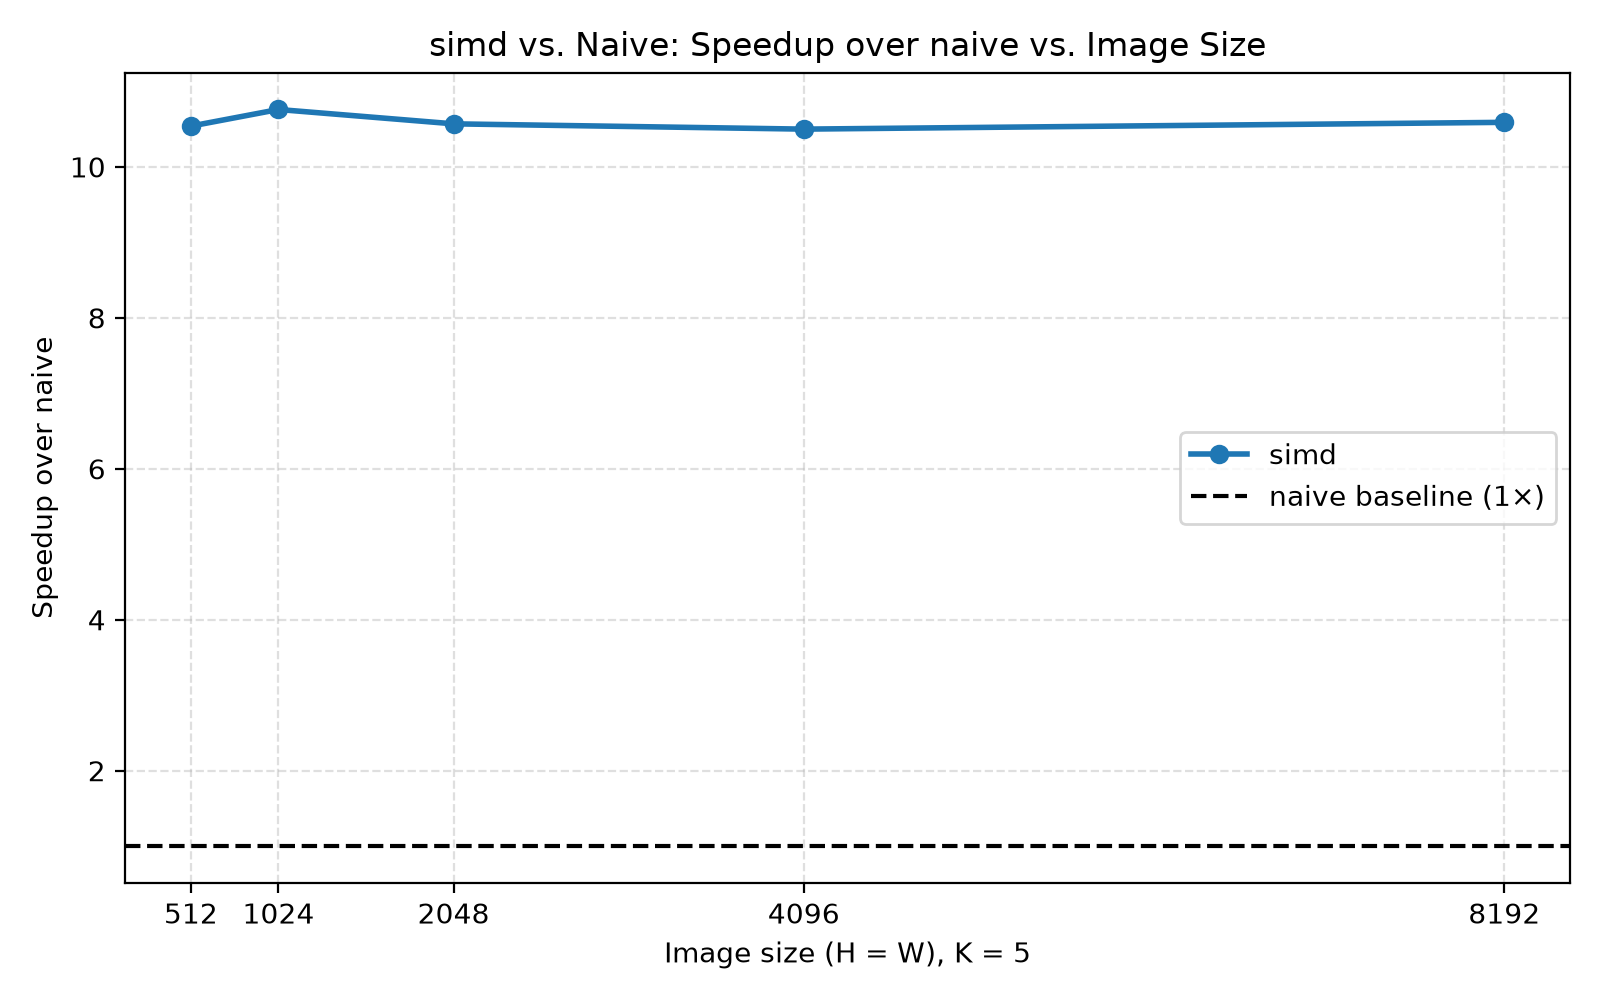
\includegraphics[width=\linewidth]{plots/task1c/simd_vs_naive_speedup_image_size_k5.png}
        \caption{Speedup vs. Image Size ($K=5$)}
    \end{subfigure}
    \hfill
    \begin{subfigure}{0.48\textwidth}
        \centering
        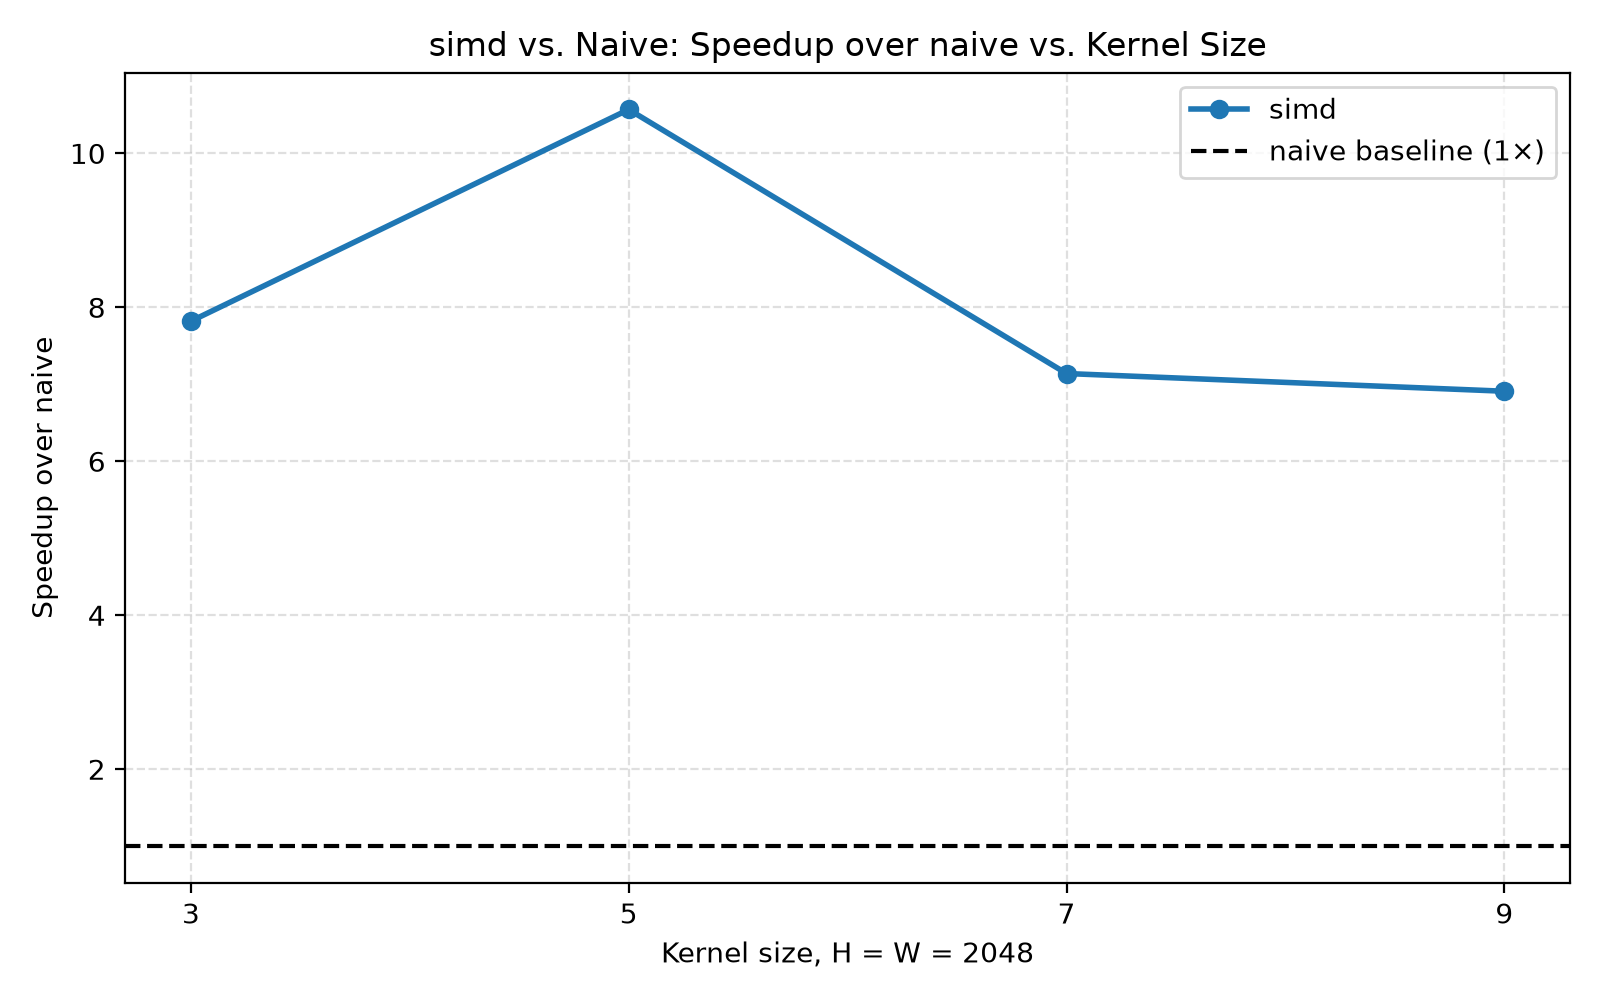
\includegraphics[width=\linewidth]{plots/task1c/simd_vs_naive_speedup_kernel_size_2048.png}
        \caption{Speedup vs. Kernel Size ($2048 \times 2048$)}
    \end{subfigure}
    
    \vspace{1em}
    \begin{subfigure}{0.48\textwidth}
        \centering
        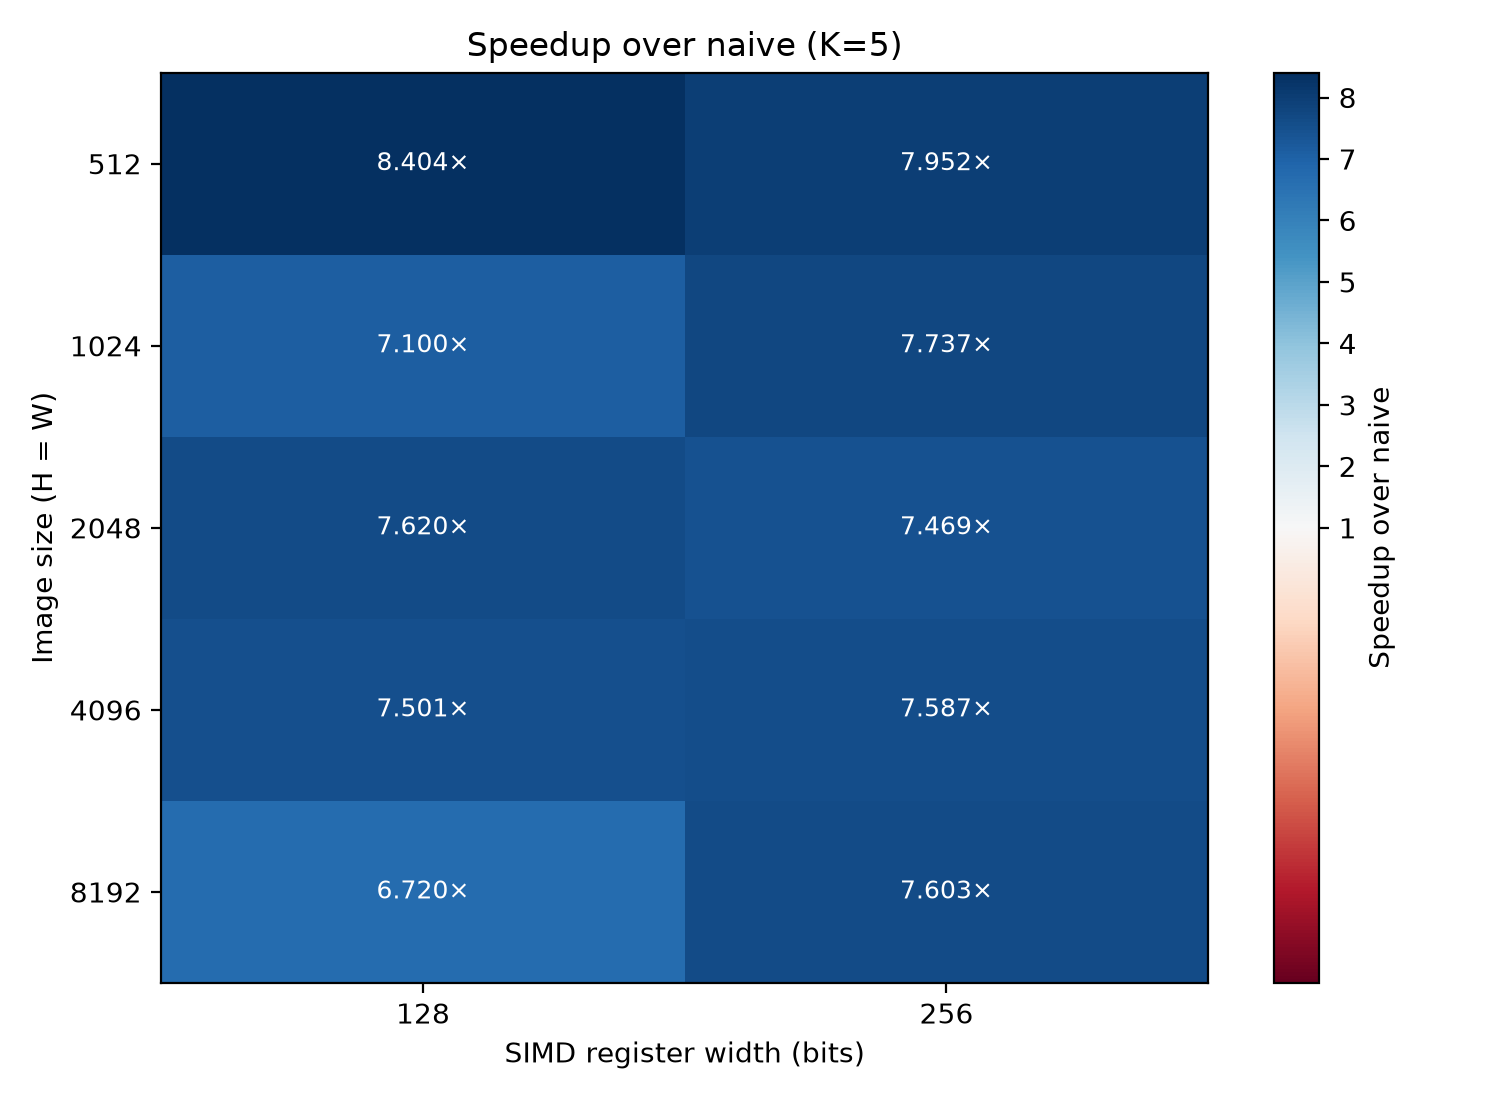
\includegraphics[width=\linewidth]{plots/task1c/speedup_heatmap_k5.png}
        \caption{Speedup Heatmap (Width vs Image Size)}
    \end{subfigure}
    \hfill
    \begin{subfigure}{0.48\textwidth}
        \centering
        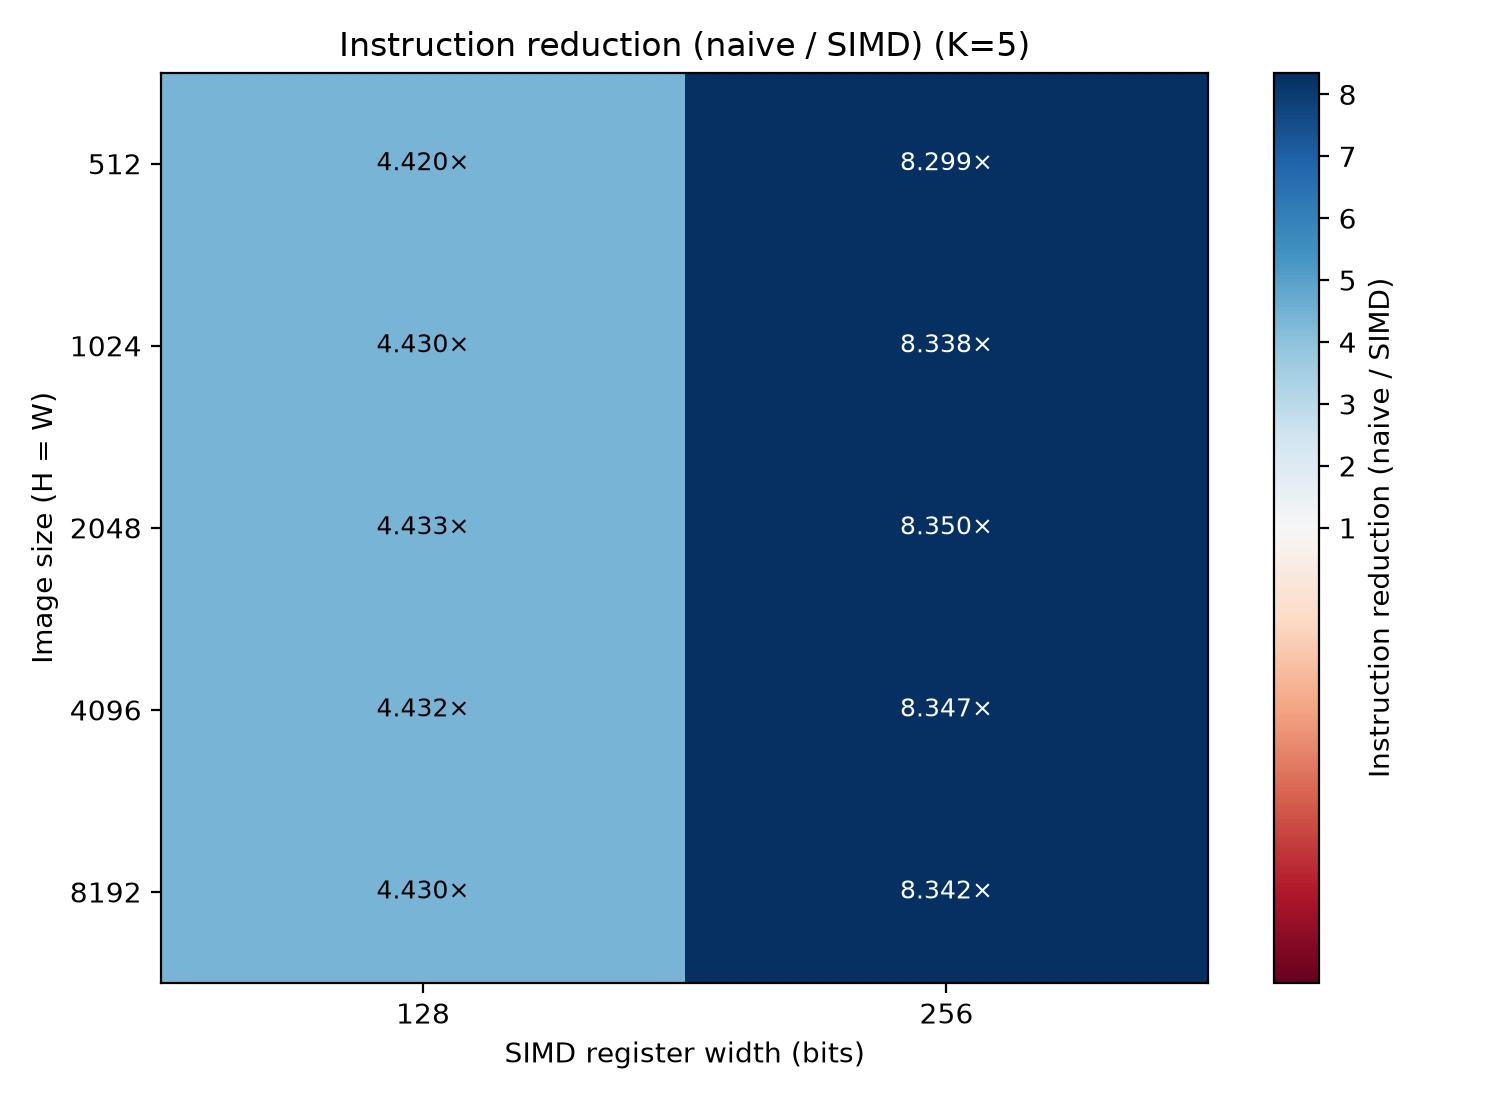
\includegraphics[width=\linewidth]{plots/task1c/instruction_reduction_heatmap_k5.png}
        \caption{Instruction Reduction Factor}
    \end{subfigure}
    \caption{SIMD performance and hardware metric improvements.}
\end{figure}

\subsection{Analysis}
SIMD substantially reduced the executed instruction count. A 128-bit vector instruction processes 4 single-precision values, while a 256-bit AVX2 vector instruction processes 8. The measured instruction reductions were approximately $4.4\times$ and $8.3\times$, respectively; realized performance also depends on loads, scheduling, and reduction overhead.

Interestingly, while 256-bit SIMD approximately halved the instructions compared to 128-bit, the raw speedup did not double. At a $1024 \times 1024$ image size, 256-bit offered a marginal speedup advantage over 128-bit ($7.74\times$ vs $7.10\times$). This indicates that data-delivery throughput and other memory-system effects become more important than arithmetic instruction count alone. Bandwidth and cache latency are distinct effects, and these measurements do not isolate either one.

\subsection{Questions}

\begin{enumerate}
    \item \textbf{How did the instruction count change?} \\
    The instruction count fell by $\sim$4.4 for the 128-bit version and $\sim$8.3 for the 256-bit version compared with the naive baseline. These reductions are consistent with processing 4 and 8 floats per vector instruction, respectively.
    \item \textbf{Did you achieve speedup? Why?} \\
    Yes, speedups of roughly $7\times$ to $8\times$ were observed. Data parallelism, fused vector multiply-add instructions, and lower loop-control overhead all contributed; the vector width specifies elements per instruction, not a guaranteed number of elements per cycle.
    \item \textbf{Which SIMD intrinsics were used and why?} \\
    We primarily used \texttt{\_mm256\_loadu\_ps} for safe unaligned memory reads, \texttt{\_mm256\_set1\_ps} to broadcast scalar weights to all vector lanes, and \texttt{\_mm256\_fmadd\_ps} for the core fused accumulation. The unaligned operations avoid requiring every sliding-window address to be 32-byte aligned.
\end{enumerate}

% ============================================================
% 1D
% ============================================================

\section{Task 1D: Combined Optimization}

\subsection{Combined Optimization}
For our final optimized implementation, we combined five techniques:
\begin{enumerate}
    \item \textbf{Cache Tiling:} We blocked the output matrix into $32 \times 32$ spatial tiles (\texttt{oyT}, \texttt{oxT}) to restrict the active memory working set .
    \item \textbf{Loop Reordering:} Within each tile, we inverted the naive loop order to \texttt{ky} $\rightarrow$ \texttt{kx} $\rightarrow$ \texttt{oy} $\rightarrow$ \texttt{ox}, ensuring that the innermost memory accesses across the \texttt{ox} dimension are perfectly sequential .
    \item \textbf{SIMD Vectorization (AVX2):} We parallelized the innermost \texttt{ox} loop using 256-bit AVX2 vectors (\texttt{\_mm256\_loadu\_ps} and \texttt{\_mm256\_fmadd\_ps}), processing 8 pixels simultaneously .
    \item \textbf{Loop Unrolling (\texttt{kx}):} We unrolled the inner \texttt{kx} loop by a factor of 2, handling two adjacent kernel columns per iteration to further reduce branch overhead .
    \item \textbf{Multiple Independent Accumulators:} Inside the vector loop, we unrolled the \texttt{oy} dimension by 4, utilizing 4 independent AVX2 accumulators (\texttt{acc0} to \texttt{acc3}) to process a $4 \times 8$ block of output pixels simultaneously, maximizing instruction-level parallelism .
\end{enumerate}

\subsection{Why Combine These Techniques?}
The techniques address different parts of the execution. Tiling improves temporal locality and increases the chance that reused data are served from the cache hierarchy. Reordering makes the innermost \texttt{ox} accesses unit-stride, while SIMD increases the amount of arithmetic performed per vector instruction. Loop unrolling and multiple accumulators reduce loop-control work and expose independent operations. The measured combined speedup reflects their joint effect; it does not isolate a single bottleneck.

\subsection{Final Performance Comparison}

\begin{figure}[H]
    \centering
    \begin{subfigure}{0.85\textwidth}
        \centering
        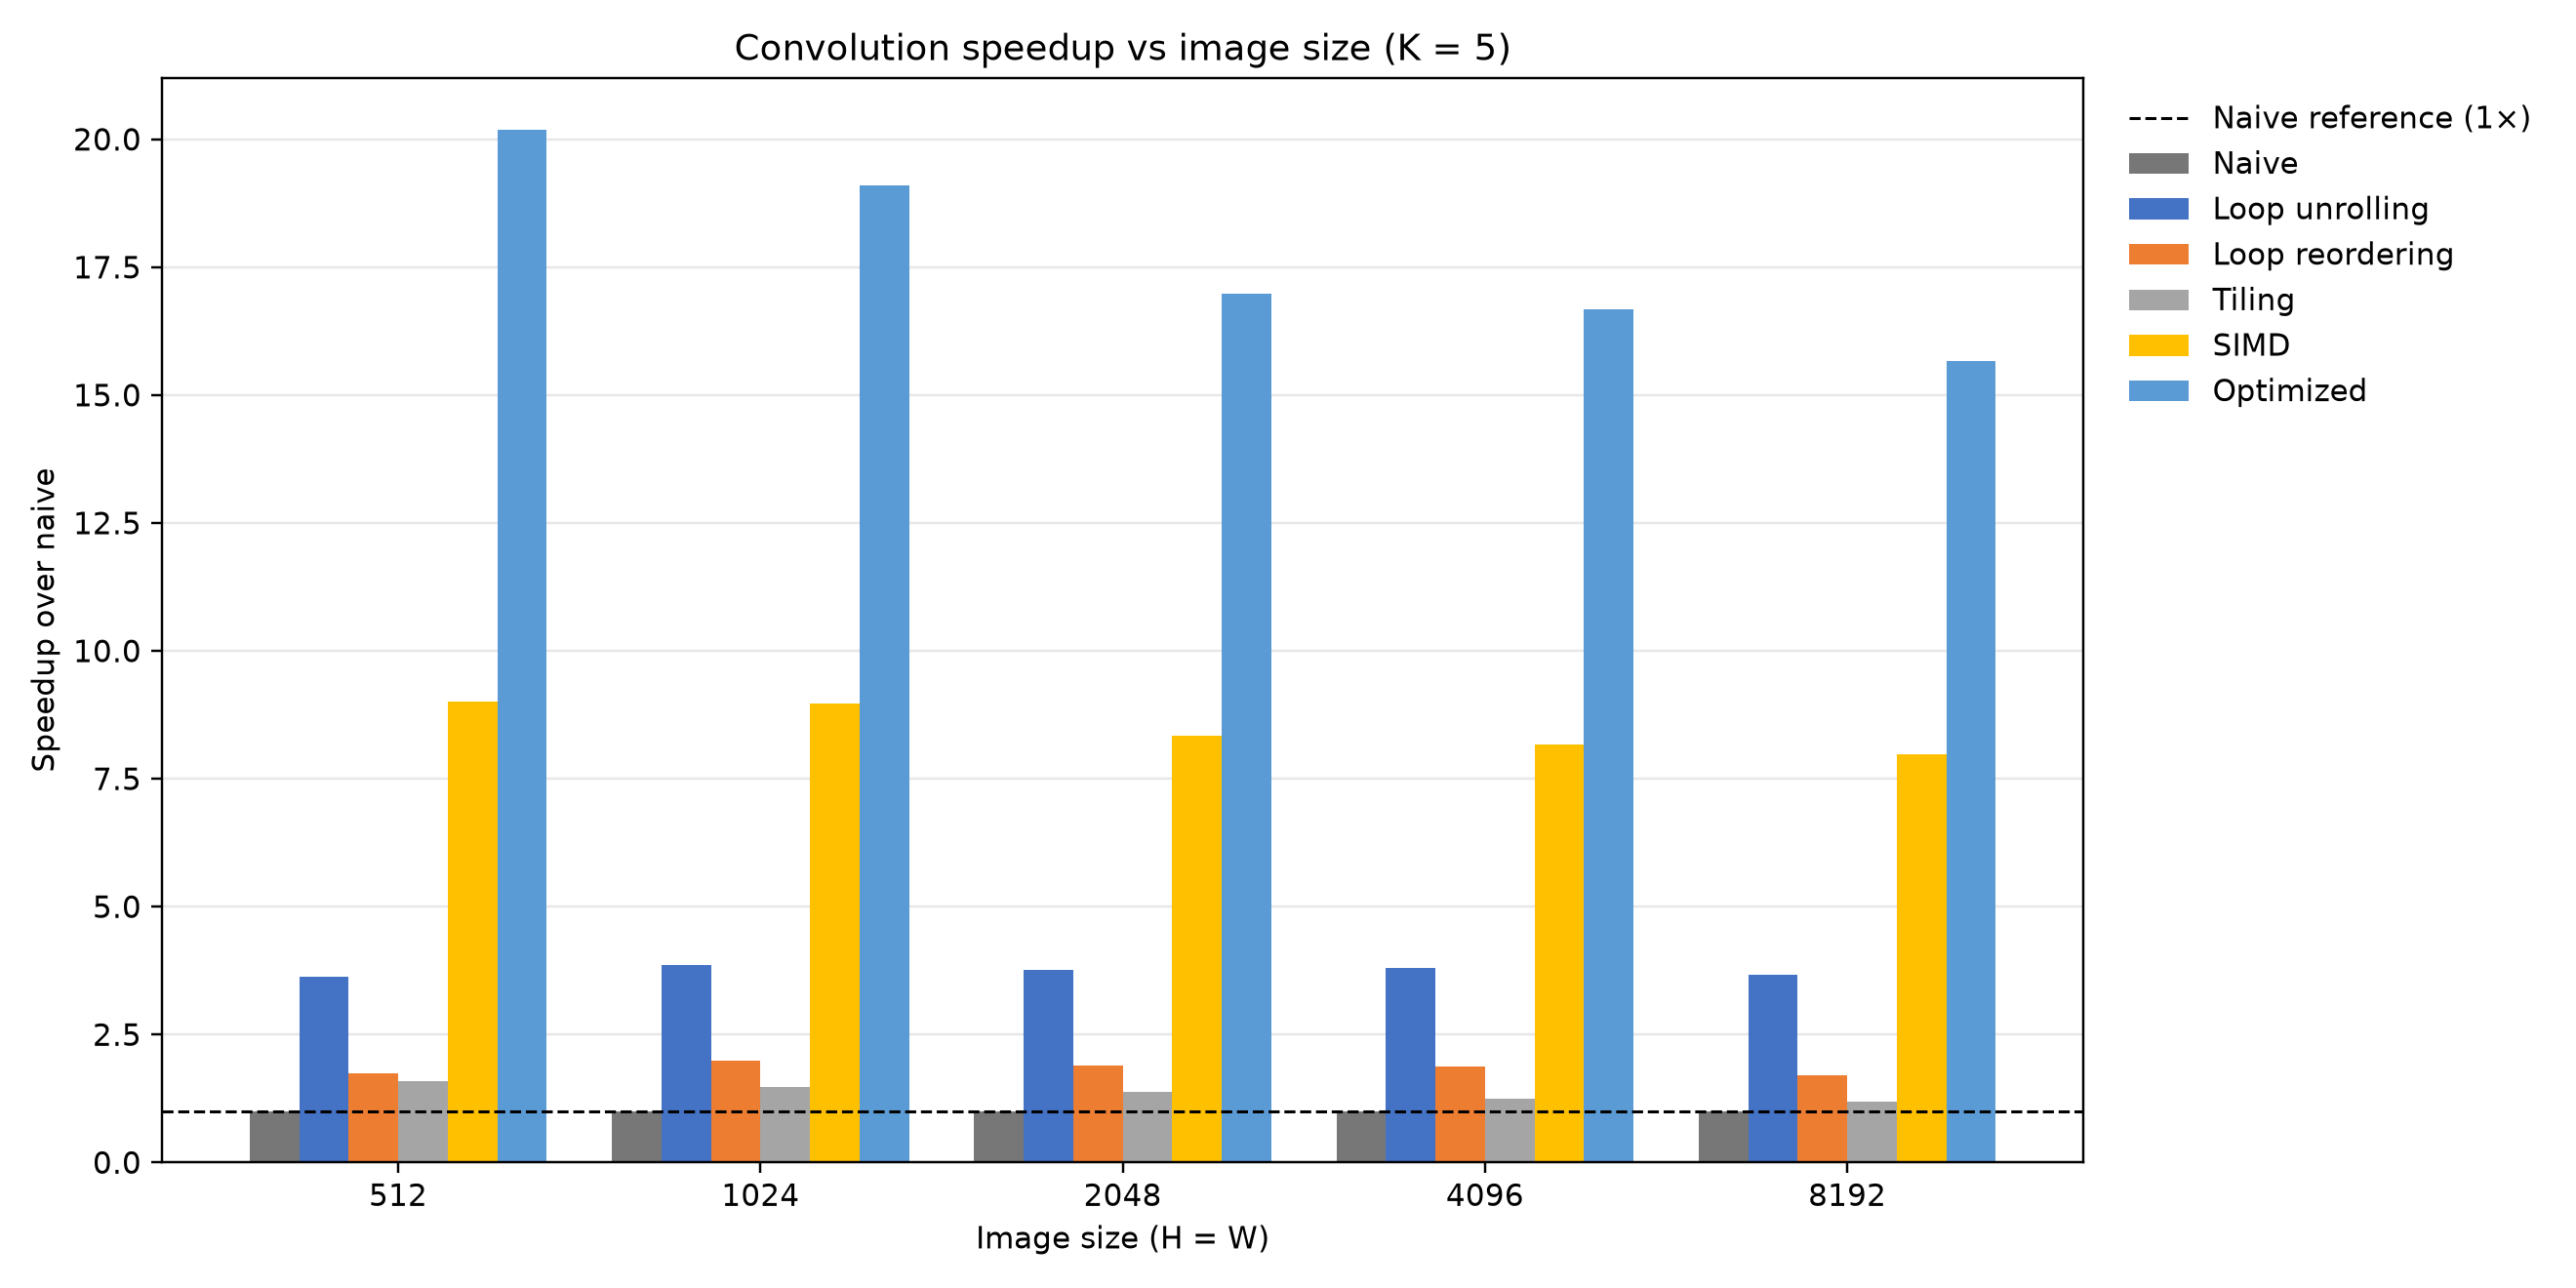
\includegraphics[width=\linewidth]{plots/task1d/speedup_vs_image_size.png}
        \caption{Speedup vs. Image Size ($K=5$)}
        \label{fig:task1d_image_size}
    \end{subfigure}
    
    \begin{subfigure}{0.85\textwidth}
        \centering
        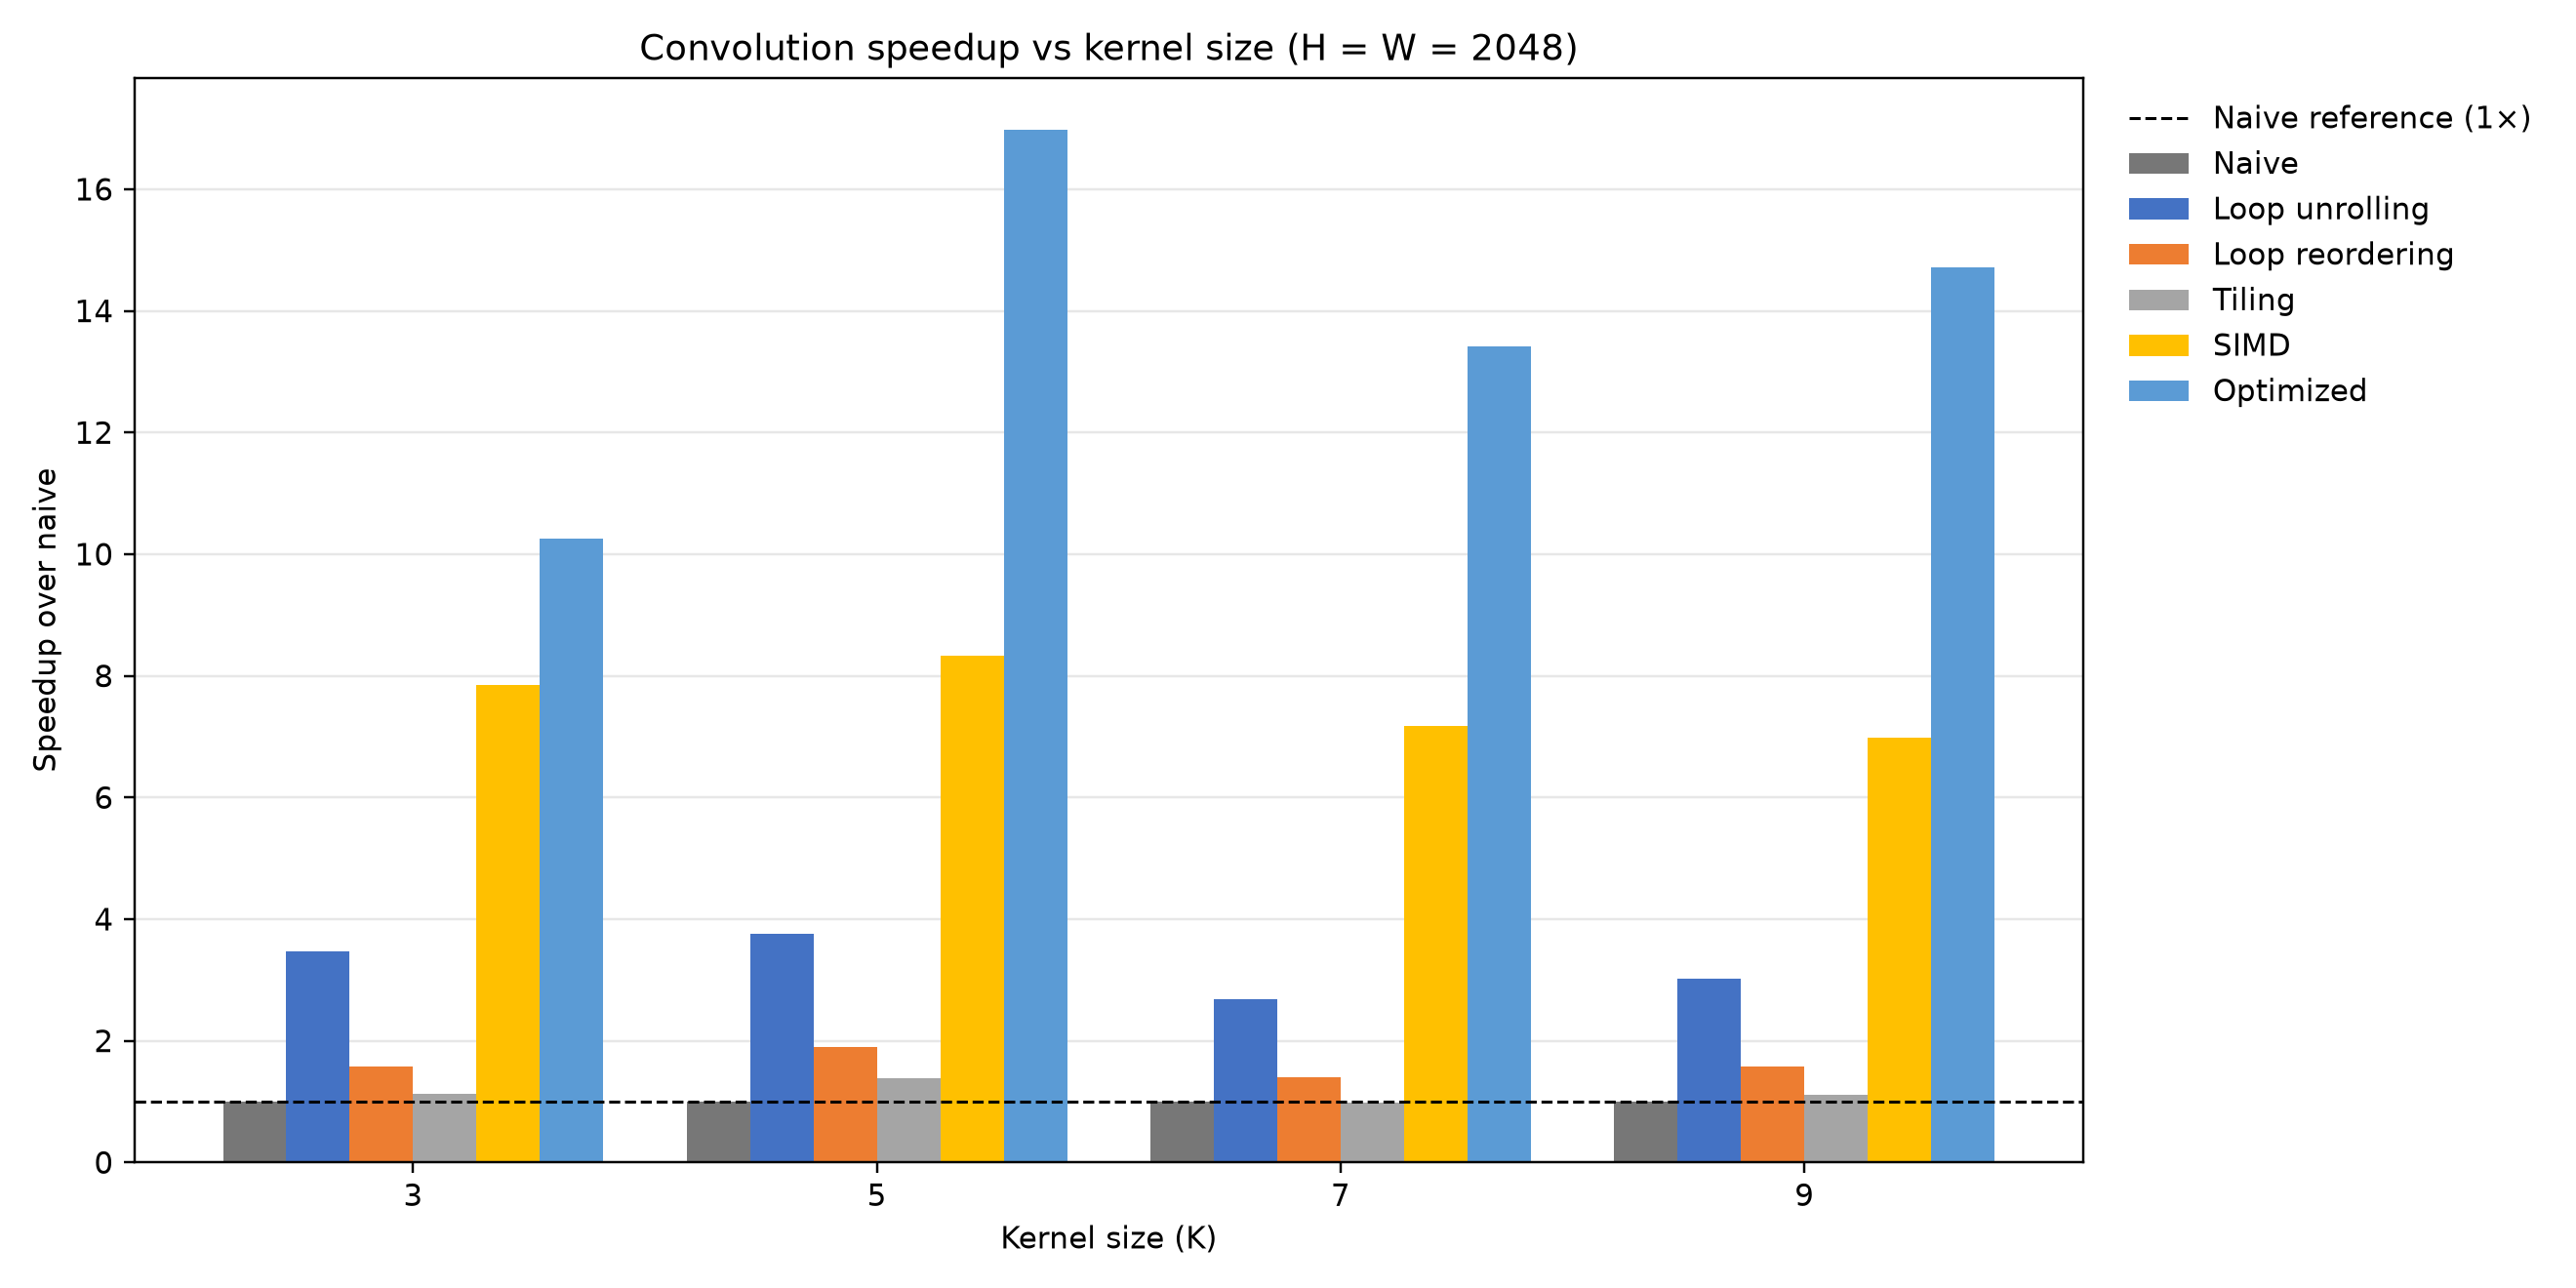
\includegraphics[width=\linewidth]{plots/task1d/speedup_vs_kernel_size.png}
        \caption{Speedup vs. Kernel Size ($2048 \times 2048$)}
        \label{fig:task1d_kernel_size}
    \end{subfigure}
    \caption{Best performance of the Task 1 optimization techniques.}
    \label{fig:task1_final_comparison}
\end{figure}

\begin{table}[H]
\centering
\caption{Task 1 final performance summary}
\begin{tabular}{lccl}
\toprule
Technique & Best Speedup & Workload & Primary Hardware Target \\
\midrule
Tiling & 1.60$\times$ & $512 \times 512, K=5$ & Cache capacity / L2+LLC hit rate \\
Loop reordering & 1.99$\times$ & $1024 \times 1024, K=5$ & Spatial locality / Hardware prefetching \\
Loop unrolling & 3.85$\times$ & $1024 \times 1024, K=5$ & Branch prediction / Loop overhead \\
SIMD (AVX2) & 9.01$\times$ & $512 \times 512, K=5$ & ALU saturation / Data parallelism \\
\textbf{Optimized (All Combined)} & \textbf{20.19$\times$} & $512 \times 512, K=5$ & \textbf{Cache locality / SIMD} \\
\bottomrule
\end{tabular}
\end{table}

\subsection{Discussion}
The combined implementation reaches a peak speedup of $20.19\times$, compared with the best isolated SIMD result of $9.01\times$. This improvement is consistent with combining vector arithmetic with improved locality and reduced loop overhead. The measurements show the combined effect, but do not by themselves prove that one specific memory bottleneck was eliminated or that the vector units reached a theoretical limit.

\subsection{Task 1 Conclusion}
Task 1 shows that loop structure and data layout matter alongside arithmetic complexity. Reordering improves unit-stride access, tiling improves reuse over a limited working set, unrolling reduces loop-control work and exposes independent operations, and SIMD raises the amount of work per vector instruction. Their combination produced the best result on the measured workloads.


\end{document}
